\documentclass[11pt % Font size
              ]{article}
\usepackage[ a4paper % Paper size and format
           , onecolumn % Number of columns: onecolumn or twocolumn
           , total={6in, 8in} % Text area: {width, height}
           ]{geometry}

\title{A Model Theoretic Study \\ of Allen's Interval Algebra}
\author{Bruno da Rocha Paiva}
\date{} % Date of writing: empty, today or 25.12.00

% Language and font encodings
\usepackage[english]{babel}
\usepackage[utf8x]{inputenc}
\usepackage[T1]{fontenc}

\usepackage[hidelinks]{hyperref}
\usepackage{fancyhdr}
\usepackage{array}
\usepackage{amsmath}
\usepackage{amsthm}
\usepackage{amssymb}
\usepackage{graphicx}
\usepackage{parskip}
\usepackage{setspace}
\usepackage[colorinlistoftodos]{todonotes}
\usepackage{tikz}
\usetikzlibrary{decorations.pathreplacing,calligraphy}
\usepackage{quiver}
\usepackage{xcolor}
\usepackage[capitalise]{cleveref}
\usepackage{algorithm}
\usepackage{algpseudocode}
\usepackage{multirow}
\usepackage{rotating}
\usepackage[numbers]{natbib}

% Used to scale tikz-cd diagrams properly
\tikzcdset{scale cd/.style={every label/.append style={scale=#1},
    cells={nodes={scale=#1}}}}

% General Symbols
\newcommand{\N}{\mathbb{N}}
\newcommand{\Z}{\mathbb{Z}}
\newcommand{\Q}{\mathbb{Q}}
\newcommand{\R}{\mathbb{R}}
\newcommand{\congto}{\xrightarrow{\sim}}
\newcommand{\letin}[2]{\text{let }{#1}\text{ in }{#2}}
\newcommand{\C}{\mathcal{C}}
\newcommand{\PS}{\mathcal{P}}

% Category Theory
\newcommand{\id}[1]{\text{id}_{#1}}
\newcommand{\unit}[1]{\eta_{#1}}
\newcommand{\counit}[1]{\epsilon_{#1}}

% Model Theory
\newcommand{\lang}{\mathcal{L}}
\newcommand{\theory}{\mathbb{T}}
\DeclareMathOperator{\age}{Age}
\DeclareMathOperator{\fulltheory}{Th}

\newcommand{\finslo}{\textbf{FCh}}
\newcommand{\finaia}{\textbf{FIA}}


\newcommand{\lslo}{\lang_\text{SLO}}
\newcommand{\tslo}{\theory_\text{SLO}}

% Allen Interval Algebra Symbols
\newcommand{\laia}{\lang_\text{AIA}}
\newcommand{\taia}{\theory_\text{AIA}}
\newcommand{\istart}[1]{#1_{-}}
\newcommand{\iend}[1]{#1_{+}}
\newcommand{\aiaindex}{\{<,m,o,s,f,d\}}

% Allen Interval Algebra Relations
\newcommand{\aiaarrow}[1]{\xrightarrow{\;#1\;}}
\newcommand{\raiaarrow}[1]{\xleftarrow{\;#1\;}}
\newcommand{\before}{\aiaarrow{<}}
\newcommand{\meets}{\aiaarrow{m}}
\newcommand{\overlaps}{\aiaarrow{o}}
\newcommand{\starts}{\aiaarrow{s}}
\newcommand{\finishes}{\aiaarrow{f}}
\newcommand{\contained}{\aiaarrow{d}}
\newcommand{\after}{\raiaarrow{<}}
\newcommand{\metby}{\raiaarrow{m}}
\newcommand{\overlappedby}{\raiaarrow{o}}
\newcommand{\startedby}{\raiaarrow{s}}
\newcommand{\finishedby}{\raiaarrow{f}}
\newcommand{\contains}{\raiaarrow{d}}

% Categories of models
\newcommand{\mods}[2]{\text{Mod}\left(#1,#2\right)}
\newcommand{\aias}{\textbf{AIA}}
\newcommand{\slos}{\textbf{SLO}}

% Intervals construction
\newcommand{\inter}[1][-]{\text{Int}\left(#1\right)}
\newcommand{\defformula}[1]{\phi_{#1}}
\newcommand{\beforef}{\defformula{\before}}
\newcommand{\meetsf}{\defformula{\meets}}
\newcommand{\overlapsf}{\defformula{\overlaps}}
\newcommand{\startsf}{\defformula{\starts}}
\newcommand{\finishesf}{\defformula{\finishes}}
\newcommand{\containedf}{\defformula{\contained}}

\newcommand{\allints}{\defformula{\text{full}}}
\newcommand{\mostints}{\defformula{\text{fullish}}}
\newcommand{\lexord}{\defformula{\text{lex}}}

% Points construction
\newcommand{\psim}{\sim}
\newcommand{\peq}{\phi_\sim}
\newcommand{\plt}{\phi_<}
\newcommand{\points}[1][-]{\text{Pts}\left(#1\right)}

% Environments
\theoremstyle{plain}
\newtheorem{thm}{Theorem}[section]
\newtheorem{lemma}[thm]{Lemma}
\newtheorem{prop}[thm]{Proposition}
\newtheorem{cor}[thm]{Corollary}

\theoremstyle{definition}
\newtheorem{defn}[thm]{Definition}
\newtheorem{exmp}[thm]{Example}

\theoremstyle{remark}
\newtheorem*{rem}{Remark}

\newcommand{\transreltable}[3]{
  \begin{table}[ht]
    \centering
    \begin{tabular}{| c | c | c || c | c | c |}
      \hline
      $I \longrightarrow J$ & $J \longrightarrow K$ & $I \longrightarrow K$ &
        $I \longrightarrow J$ & $J \longrightarrow K$ & $I \longrightarrow K$ \\
      \hline\hline
      #3
      \hline
    \end{tabular}
    \caption{#2}
    \label{tab:#1}
  \end{table}
}

\newcommand{\llrow}{$<$ & $<$ & $<$}
\newcommand{\lmrow}{$<$ & $m$ & $<$}
\newcommand{\lorow}{$<$ & $o$ & $<$}
\newcommand{\lsrow}{$<$ & $s$ & $<$}
\newcommand{\lfrow}{$<$ & $f$ & $<mosd$}
\newcommand{\ldrow}{$<$ & $d$ & $<mosd$}
\newcommand{\lerow}{$<$ & $=$ & $<$}
\newcommand{\lLrow}{$<$ & $>$ & full}
\newcommand{\lMrow}{$<$ & $M$ & $<mosd$}
\newcommand{\lOrow}{$<$ & $O$ & $<mosd$}
\newcommand{\lSrow}{$<$ & $S$ & $<$}
\newcommand{\lFrow}{$<$ & $F$ & $<$}
\newcommand{\lDrow}{$<$ & $D$ & $<$}

\newcommand{\mlrow}{$m$ & $<$ & $<$}
\newcommand{\mmrow}{$m$ & $m$ & $<$}
\newcommand{\morow}{$m$ & $o$ & $<$}
\newcommand{\msrow}{$m$ & $s$ & $m$}
\newcommand{\mfrow}{$m$ & $f$ & $osd$}
\newcommand{\mdrow}{$m$ & $d$ & $osd$}
\newcommand{\merow}{$m$ & $=$ & $m$}
\newcommand{\mLrow}{$m$ & $>$ & $>MOSD$}
\newcommand{\mMrow}{$m$ & $M$ & $f=F$}
\newcommand{\mOrow}{$m$ & $O$ & $osd$}
\newcommand{\mSrow}{$m$ & $S$ & $m$}
\newcommand{\mFrow}{$m$ & $F$ & $<$}
\newcommand{\mDrow}{$m$ & $D$ & $<$}

\newcommand{\olrow}{$o$ & $<$ & $<$}
\newcommand{\omrow}{$o$ & $m$ & $<$}
\newcommand{\oorow}{$o$ & $o$ & $<mo$}
\newcommand{\osrow}{$o$ & $s$ & $o$}
\newcommand{\ofrow}{$o$ & $f$ & $osd$}
\newcommand{\odrow}{$o$ & $d$ & $osd$}
\newcommand{\oerow}{$o$ & $=$ & $o$}
\newcommand{\oLrow}{$o$ & $>$ & $>MOSD$}
\newcommand{\oMrow}{$o$ & $M$ & $OSD$}
\newcommand{\oOrow}{$o$ & $O$ & concur}
\newcommand{\oSrow}{$o$ & $S$ & $oFD$}
\newcommand{\oFrow}{$o$ & $F$ & $<mo$}
\newcommand{\oDrow}{$o$ & $D$ & $<moFD$}

\newcommand{\slrow}{$s$ & $<$ & $<$}
\newcommand{\smrow}{$s$ & $m$ & $<$}
\newcommand{\sorow}{$s$ & $o$ & $<mo$}
\newcommand{\ssrow}{$s$ & $s$ & $s$}
\newcommand{\sfrow}{$s$ & $f$ & $d$}
\newcommand{\sdrow}{$s$ & $d$ & $d$}
\newcommand{\serow}{$s$ & $=$ & $s$}
\newcommand{\sLrow}{$s$ & $>$ & $>$}
\newcommand{\sMrow}{$s$ & $M$ & $M$}
\newcommand{\sOrow}{$s$ & $O$ & $fdO$}
\newcommand{\sSrow}{$s$ & $S$ & $s=S$}
\newcommand{\sFrow}{$s$ & $F$ & $<mo$}
\newcommand{\sDrow}{$s$ & $D$ & $<moFD$}

\newcommand{\flrow}{$f$ & $<$ & $<$}
\newcommand{\fmrow}{$f$ & $m$ & $m$}
\newcommand{\forow}{$f$ & $o$ & $osd$}
\newcommand{\fsrow}{$f$ & $s$ & $d$}
\newcommand{\ffrow}{$f$ & $f$ & $f$}
\newcommand{\fdrow}{$f$ & $d$ & $d$}
\newcommand{\ferow}{$f$ & $=$ & $f$}
\newcommand{\fLrow}{$f$ & $>$ & $>$}
\newcommand{\fMrow}{$f$ & $M$ & $>$}
\newcommand{\fOrow}{$f$ & $O$ & $>MO$}
\newcommand{\fSrow}{$f$ & $S$ & $>MO$}
\newcommand{\fFrow}{$f$ & $F$ & $f=F$}
\newcommand{\fDrow}{$f$ & $D$ & $>MOSD$}

\newcommand{\dlrow}{$d$ & $<$ & $<$}
\newcommand{\dmrow}{$d$ & $m$ & $<$}
\newcommand{\dorow}{$d$ & $o$ & $<mosd$}
\newcommand{\dsrow}{$d$ & $s$ & $d$}
\newcommand{\dfrow}{$d$ & $f$ & $d$}
\newcommand{\ddrow}{$d$ & $d$ & $d$}
\newcommand{\derow}{$d$ & $=$ & $d$}
\newcommand{\dLrow}{$d$ & $>$ & $>$}
\newcommand{\dMrow}{$d$ & $M$ & $>$}
\newcommand{\dOrow}{$d$ & $O$ & $df>OM$}
\newcommand{\dSrow}{$d$ & $S$ & $df>OM$}
\newcommand{\dFrow}{$d$ & $F$ & $<mosd$}
\newcommand{\dDrow}{$d$ & $D$ & full}

\newcommand{\elrow}{$=$ & $<$ & $<$}
\newcommand{\emrow}{$=$ & $m$ & $m$}
\newcommand{\eorow}{$=$ & $o$ & $o$}
\newcommand{\esrow}{$=$ & $s$ & $s$}
\newcommand{\efrow}{$=$ & $f$ & $f$}
\newcommand{\edrow}{$=$ & $d$ & $d$}
\newcommand{\eerow}{$=$ & $=$ & $=$}
\newcommand{\eLrow}{$=$ & $>$ & $>$}
\newcommand{\eMrow}{$=$ & $M$ & $M$}
\newcommand{\eOrow}{$=$ & $O$ & $O$}
\newcommand{\eSrow}{$=$ & $S$ & $S$}
\newcommand{\eFrow}{$=$ & $F$ & $F$}
\newcommand{\eDrow}{$=$ & $D$ & $D$}

\newcommand{\Llrow}{$>$ & $<$ & full}
\newcommand{\Lmrow}{$>$ & $m$ & $df>OM$}
\newcommand{\Lorow}{$>$ & $o$ & $df>OM$}
\newcommand{\Lsrow}{$>$ & $s$ & $df>OM$}
\newcommand{\Lfrow}{$>$ & $f$ & $>$}
\newcommand{\Ldrow}{$>$ & $d$ & $df>OM$}
\newcommand{\Lerow}{$>$ & $=$ & $>$}
\newcommand{\LLrow}{$>$ & $>$ & $>$}
\newcommand{\LMrow}{$>$ & $M$ & $>$}
\newcommand{\LOrow}{$>$ & $O$ & $>$}
\newcommand{\LSrow}{$>$ & $S$ & $>$}
\newcommand{\LFrow}{$>$ & $F$ & $>$}
\newcommand{\LDrow}{$>$ & $D$ & $>$}

\newcommand{\Mlrow}{$M$ & $<$ & $<moFD$}
\newcommand{\Mmrow}{$M$ & $m$ & $s=S$}
\newcommand{\Morow}{$M$ & $o$ & $fdO$}
\newcommand{\Msrow}{$M$ & $s$ & $fdO$}
\newcommand{\Mfrow}{$M$ & $f$ & $M$}
\newcommand{\Mdrow}{$M$ & $d$ & $fdO$}
\newcommand{\Merow}{$M$ & $=$ & $M$}
\newcommand{\MLrow}{$M$ & $>$ & $>$}
\newcommand{\MMrow}{$M$ & $M$ & $>$}
\newcommand{\MOrow}{$M$ & $O$ & $>$}
\newcommand{\MSrow}{$M$ & $S$ & $>$}
\newcommand{\MFrow}{$M$ & $F$ & $M$}
\newcommand{\MDrow}{$M$ & $D$ & $>$}

\newcommand{\Olrow}{$O$ & $<$ & $<moFD$}
\newcommand{\Omrow}{$O$ & $m$ & $oFD$}
\newcommand{\Oorow}{$O$ & $o$ & concur}
\newcommand{\Osrow}{$O$ & $s$ & $fdO$}
\newcommand{\Ofrow}{$O$ & $f$ & $O$}
\newcommand{\Odrow}{$O$ & $d$ & $fdO$}
\newcommand{\Oerow}{$O$ & $=$ & $O$}
\newcommand{\OLrow}{$O$ & $>$ & $>$}
\newcommand{\OMrow}{$O$ & $M$ & $>$}
\newcommand{\OOrow}{$O$ & $O$ & $>MO$}
\newcommand{\OSrow}{$O$ & $S$ & $>MO$}
\newcommand{\OFrow}{$O$ & $F$ & $OSD$}
\newcommand{\ODrow}{$O$ & $D$ & $>MOSD$}

\newcommand{\Slrow}{$S$ & $<$ & $<moFD$}
\newcommand{\Smrow}{$S$ & $m$ & $oFD$}
\newcommand{\Sorow}{$S$ & $o$ & $oFD$}
\newcommand{\Ssrow}{$S$ & $s$ & $s=S$}
\newcommand{\Sfrow}{$S$ & $f$ & $O$}
\newcommand{\Sdrow}{$S$ & $d$ & $fdO$}
\newcommand{\Serow}{$S$ & $=$ & $S$}
\newcommand{\SLrow}{$S$ & $>$ & $>$}
\newcommand{\SMrow}{$S$ & $M$ & $M$}
\newcommand{\SOrow}{$S$ & $O$ & $O$}
\newcommand{\SSrow}{$S$ & $S$ & $S$}
\newcommand{\SFrow}{$S$ & $F$ & $D$}
\newcommand{\SDrow}{$S$ & $D$ & $D$}

\newcommand{\Flrow}{$F$ & $<$ & $<$}
\newcommand{\Fmrow}{$F$ & $m$ & $m$}
\newcommand{\Forow}{$F$ & $o$ & $o$}
\newcommand{\Fsrow}{$F$ & $s$ & $o$}
\newcommand{\Ffrow}{$F$ & $f$ & $f=F$}
\newcommand{\Fdrow}{$F$ & $d$ & $osd$}
\newcommand{\Ferow}{$F$ & $=$ & $F$}
\newcommand{\FLrow}{$F$ & $>$ & $>MOSD$}
\newcommand{\FMrow}{$F$ & $M$ & $OSD$}
\newcommand{\FOrow}{$F$ & $O$ & $OSD$}
\newcommand{\FSrow}{$F$ & $S$ & $D$}
\newcommand{\FFrow}{$F$ & $F$ & $F$}
\newcommand{\FDrow}{$F$ & $D$ & $D$}

\newcommand{\Dlrow}{$D$ & $<$ & $<moFD$}
\newcommand{\Dmrow}{$D$ & $m$ & $oFD$}
\newcommand{\Dorow}{$D$ & $o$ & $oFD$}
\newcommand{\Dsrow}{$D$ & $s$ & $oFD$}
\newcommand{\Dfrow}{$D$ & $f$ & $OSD$}
\newcommand{\Ddrow}{$D$ & $d$ & concur}
\newcommand{\Derow}{$D$ & $=$ & $D$}
\newcommand{\DLrow}{$D$ & $>$ & $>MOSD$}
\newcommand{\DMrow}{$D$ & $M$ & $OSD$}
\newcommand{\DOrow}{$D$ & $O$ & $OSD$}
\newcommand{\DSrow}{$D$ & $S$ & $D$}
\newcommand{\DFrow}{$D$ & $F$ & $D$}
\newcommand{\DDrow}{$D$ & $D$ & $D$}

\begin{document}
\pagestyle{empty}
\begin{titlepage}

\newcommand{\HRule}{\rule{\linewidth}{0.5mm}} % Defines a new command for the horizontal lines, change thickness here

%----------------------------------------------------------------------------------------
%	LOGO SECTION
%----------------------------------------------------------------------------------------


\includegraphics[width=8cm]{title/logo.eps}\\[1cm] % Include a department/university logo - this will require the graphicx package

%----------------------------------------------------------------------------------------

\center % Center everything on the page

%----------------------------------------------------------------------------------------
%	HEADING SECTIONS
%----------------------------------------------------------------------------------------

\textsc{\LARGE MEng Individual Project}\\[1.5cm] % Name of your university/college
\textsc{\Large Imperial College London}\\[0.5cm] % Major heading such as course name
\textsc{\large Department of Computing}\\[0.5cm] % Minor heading such as course title

%----------------------------------------------------------------------------------------
%	TITLE SECTION
%----------------------------------------------------------------------------------------
\makeatletter
\HRule \\[0.4cm]
{ \huge \bfseries \@title}\\[0.4cm] % Title of your document
\HRule \\[1.5cm]

%----------------------------------------------------------------------------------------
%	AUTHOR SECTION
%----------------------------------------------------------------------------------------

\begin{minipage}{0.4\textwidth}
\begin{flushleft} \large
\emph{Author:}\\
\@author % Your name
\end{flushleft}
\end{minipage}
~
\begin{minipage}{0.4\textwidth}
\begin{flushright} \large
\emph{Supervisor:} \\
Dr. Robert Barham \\[1.2em] % Supervisor's Name
\emph{Second Marker:} \\
Dr. Charlotte Kestner % second marker's name
\end{flushright}
\end{minipage}\\[2cm]
\makeatother

% If you don't want a supervisor, uncomment the two lines below and remove the section above
%\Large \emph{Author:}\\
%John \textsc{Smith}\\[3cm] % Your name

%----------------------------------------------------------------------------------------
%	DATE SECTION
%----------------------------------------------------------------------------------------

{\large \today}\\[2cm] % Date, change the \today to a set date if you want to be precise

\vfill % Fill the rest of the page with whitespace

\end{titlepage}

%TODO add references to A. Pillay's notes on model theory

\newpage
\hspace{0pt}
\vfill
\begin{center}
    \textbf{Abstract}
\end{center}
Interval algebras were first introduced by Allen to reason about time intervals qualitatively. As
a result they have been mainly of interest in computer science, where their applications and
questions about decidability have been considered. However, so far they have not been studied in a
model theoretic capacity: for example pinning down their axioms and finding their out what
properties their models have.

In this report we provide a first order axiomatisation of Allen's interval algebra and we show
two constructions: the interval construction $\inter$ sending a linear order to the interval algebra
of its non-zero intervals ; and the points $\points$ construction sending an interval algebra to
the linear order of start and end points of its intervals. We show these constructions give rise to
a pair of adjoint functors, and we leverage this to show the Fraïssé limit of the finite interval
algebras is $\inter[\Q]$. From a stability theory perspective, we show that the stable interval
algebras are exactly the finite interval algebras and that for any linear order $L$, $\inter[L]$
has the non-independence property.
\vfill
\hspace{0pt}

\newpage
\hspace{0pt}
\vfill
\begin{center}
    \textbf{Acknowledgements}
\end{center}
No man is an island and this project would not have been possible without the help of many people,
for whom I wish to express my deepest gratitude.

Above all I would like to thank my supervisor Dr. Robert Barham for suggesting this topic and
giving me the much needed intuition to understand a lot of the quite technical concepts in model
theory, as well as the historical context to fully appreciate its results. I started this project
wanting to learn about model theory and I have finished it loving the subject, all thanks to
Robert's guidance.

I would also like to thank my second marker Dr. Charlotte Kestner whose feedback on my interim
report helped me flesh out the introduction and background sections, turning them into pieces of
writing I am very happy with.

Although he has not had any technical involvement with this project, I want to thank my personal
tutor Prof. Paul Kelly for the very interesting conversations we have had over the last four years,
without which I would have missed out on a lot of interesting areas.

Finally, I want to thank my parents Paulo and Paula Paiva for their endless love and support, and
my friends at Imperial College London, especially Aporva, Ben and Xueyan for acting as my
rubber duckies at multiple points in this project.

\vfill
\hspace{0pt}

\newpage
\tableofcontents

\newpage
\pagestyle{fancy}
\fancyhf{}
% \renewcommand{\sectionmark}[1]{\markboth{\thesection.\ #1}{}}
\lhead{\nouppercase{\leftmark}}
\fancyfoot[C]{\thepage}
\setlength{\headheight}{13.59999pt}
\addtolength{\topmargin}{-1.59999pt}


\section{Introduction}%
\label{sec:introduction}

\subsection{Motivation}%
\label{sub:motivation}

Model theory concerns itself with the connection between first order theories, that is
sets of axioms with universal and existential quantifiers, and the models of these
theories. The compactness theorem and the Löwenheim–Skolem theorems are examples of
significant early results in model theory, both focusing on the existence of models for a
theory: the compactness theorem saying that a model exists for a theory if models
exist for each finite fragment of the theory; and the Löwenheim–Skolem theorems telling
us that if a theory has an infinite model, then there exist models of any cardinality
greater than or equal to the number of symbols in the language.

As a consequence of the Löwenheim–Skolem theorems, we know that there exists no theory
with a unique infinite model up to isomorphism. This raises the question of what can
we say about the number of models a theory has for each cardinality.

\begin{defn}
  For a complete theory $\theory$, we write $I(\theory, \kappa)$ to mean the number of
  models, up to isomorphism, of $\theory$ with cardinality $\kappa$. We call
  $I(\theory, -)$ the spectrum of $\theory$.
\end{defn}

One of the first answers to this question came in the form of Morley's categoricity
theorem, which said that for a countable theory $\theory$, if $I(\theory,\kappa) = 1$ for
some uncountable $\kappa$, then $I(\theory,\lambda) = 1$ for all uncountable $\lambda$
\cite{10.2307/1994188}.Work by Shelah in the 1970s then extended this result to uncountable theories
\cite{Sh:31}, beginning the study of classification theory as a discipline of model theory.

Important notions from stability theory came in the form of stable and unstable theories.
Stable theories were well-behaved enough to limit the number, while in unstable theories
one always has the maximum possible number of models, that is
$I(\theory,\kappa) = 2^\kappa$ for any $\kappa > |\theory|$ \cite{Sh:a}. Being a stable theory
is a very strong condition, hence the study generalisations of stability are important.
One such generalisation, which we will discuss in this report, comes from the
non-independence property, which says that there is no formula able to pick out every
subset of an infinite subset of a model.

Classification theory is not the only active discipline of model theory however. Another
area with a lot of interesting questions comes from the study of homogeneous structures,
where any isomorphism between finite substructures can be extended to an automorphism of
the homogeneous structure. In 1953, Fraïssé showed how to construct such structures
by gluing classes of finite structures together, from which their study followed.

Hence, in the spirit of these disciplines, we will consider the first-order theory of
interval algebras, which were originally introduced by Allen in 1983 to argue about time
qualitatively, and try to find their place in the universe of model
theory, by considering their different models and how well-behaved they are.

\subsection{Report Structure}%
\label{sub:report_structure}

The rest of the report will be structured as follows. In
\cref{sec:background} we summarise the results from Allen's original paper
on interval algebras \cite{allen83}, focusing on the choices that lead to
the 13 relations and the algorithm to infer missing relations from a given
interval network. We also introduce the necessary notions from model theory
such as homogeneous models, and stable/NIP theories. We try to keep this
introduction grounded by working through some examples where possible.
Readers comfortable with these areas may safely skip them in favour of
\cref{sec:axiomatisation} and onwards.

In \cref{sec:axiomatisation} we tackle the question of axiomatisation of
interval algebras. We propose some axioms based on the understanding from
\cref{sec:axiomatisation} and show that these are satisfiable by
constructing models from linear orders. To further justify this
axiomatisation, we will then construct linear orders from interval
algebras.

In \cref{sec:adjunction} we explore further the intervals and points
constructions from \cref{sec:axiomatisation} and show they can be extended to two adjoint
functors between the relevant categories of models. We also give characterisations of
the interval algebras and linear orders for which the unit and counit are isomorphisms.
These characterisations will be expressible as first order sentences, a fact we will use
when studying the classification theory of interval algebras.

Finally, in \cref{sec:model_theory} we study the model theory of interval algebra. This
begins by considering the the class of finite interval algebras and computing its
Fraïssé limit using the machinery developed in \cref{sec:adjunction}. On the topic of
stability, we show that the stable interval algebras are exactly the finite interval
algebras. Following this there is a study of the NIP in interval algebras, for which
we find a big class of NIP algebras as well as an example of an interval algebra with the
IP.



\newpage
\section{Background}%
\label{sec:background}

\subsection{Allen's Interval Algebra}%
\label{sub:allen_interval_algebras}

The concept of Allen's interval algebras was first introduced in \cite{allen83}. The main
idea was to introduce a new system for arguing about time intervals in a qualitative way, similar
to how humans think about time. For example, when retelling a story
people will convey some ordering of events' start and end times, while skipping over the actual
figures. Now, this might happen because the specific time frames aren't relevant to the story
or even because they are not known. Regardless of the reason, it is often helpful to talk 
about time without being overly explicit. Computers however, tend to argue about time in a
quantitative manner: saving timestamps inside of logs, such that if something goes wrong, the
order of events can be gotten; checking the system clock to tell if access tokens have expired;
so on. The difficulties of expressing time qualitatively on a computer become even more obvious
when working towards artificial intelligence, for instance in natural language processing,
where the computer must be able to infer the timing of events from people's informal speech or
writing.

Interval algebras were Allen's approach to have computers reasoning about time as humans did and
still do. In an interval algebra, time intervals are treated as primitives, with binary relations
recording their ordering and level of overlap. There are 13 basic
relations which allow one to describe fully how any two intervals $I$ and $J$ might relate. The
relations and their meaning can be found in \cref{tab:basic_relations}. Apart from $=$ which is
its own dual relation, relations come in pairs of dual relations: as an example, if it is known
that $I < J$, then it can be immediately infered that $J > I$. Due to this
duality we have omitted the meaning of the dual relations from \cref{tab:basic_relations} to save
space. We have also used $\istart{I}$ and $\iend{I}$ as shorthands for the
start and end points of the interval $I$.

\begin{table}[htpb]
  \centering
  \begin{tabular}{|l|c|c|c|}
    \hline
    Relation & Symbol & Dual Symbol & Meaning \\
    \hline
    \(I\) starts \(J\)
             & \(I < J\)
             & \(I > J\)
             & \(\istart{I} < \iend{I} < \istart{J} < \iend{J}\)\\
    \(I\) meets \(J\)
             & \(I\text{ m } J\)
             & \(I\text{ M } J\)
             & \(\istart{I} < \iend{I} = \istart{J} < \iend{J}\)\\
    \(I\) overlaps \(J\)
             & \(I\text{ o } J\)
             & \(I\text{ O } J\)
             & \(\istart{I} < \istart{J} < \iend{I} < \iend{J}\)\\
    \(I\) starts \(J\)
             & \(I\text{ s } J\)
             & \(I\text{ S } J\)
             & \(\istart{J} < \istart{I} < \iend{I} < \iend{J}\)\\
    \(I\) finishes \(J\)
             & \(I\text{ f } J\)
             & \(I\text{ F } J\)
             & \(\istart{I} = \istart{J} < \iend{I} < \iend{J}\)\\
    \(I\) during \(J\)
             & \(I\text{ d } J\)
             & \(I\text{ D } J\)
             & \(\istart{J} < \istart{I} < \iend{I} = \iend{J}\)\\
    \(I\) equals \(J\)
             & \(I = J\)
             & \(I = J\)
             & \(\istart{I} = \istart{J} < \iend{I} = \iend{J}\)\\
    \hline
  \end{tabular}
  \caption{13 Basic Relations of Allen's Interval Algebra}
  \label{tab:basic_relations}
\end{table}

The choice of these 13 relations has some advantages which simplify reasoning, namely the
relations are both exhaustive and mutually-exclusive.  By exhaustive we mean that for any two
intervals $I$ and $J$, there exists at least one relation R  such that $I\text{ R }J$. By
mutually exclusive we mean there exists at most one such relation R for any two intervals $I$ and 
$J$. 

Looking at the intended meaning of each relation in \cref{tab:basic_relations} it seems that time
points are not considered as valid intervals since $\istart{I}$ is always strictly less than
$\iend{I}$. This is no accident, as time points can cause ambiguities and thus complicate the
semantics of interval algebras. This deserves some attention, since in natural language we often
refer to actual points in time instead of intervals.  For example the phrase ``I caught the ball''
suggests that the act of catching the ball was instantaneous, even though it definitely
happened over an interval of time, simply a very short one. In reality, whether we consider
certain intervals as time points or as actual intervals depends a lot on context. Furthermore,
if one really wishes to deal with time points, then they can be modelled by suitably small
intervals.

\subsubsection{Basic Algorithm}%
\label{ssub:basic_algorithm}

With some of the main ideas explained, now is a good time to see the basic algorithm described in
\cite{allen83}. It takes as input a collection of intervals and their known relations, and
attempts to infer as many of the missing relations as possible. As mentioned
before, time intervals are primitives in Allen's interval algebra and since every two intervals
must be related by one of the symbols in \cref{tab:basic_relations}, directed graphs with
labeled edges are a good representation of this information. In such a graph, there will be a node
for each time interval we are interested in, and each edge will be labelled with the sets of
symbols that describe the possible relations between the source and target intervals. Considering
an illustrative example, suppose there are two nodes $I$ and $J$ with an edge from $I$ to $J$
labelled by ``<mo'': this should be read as saying that one of $I < J$, $I\text{ m }J$ or
$I\text{ o }J$ is expected to hold, although we do not know which one.
This labelling takes advantage of the fact that all the basic relations
are mutually exclusive, so the implied disjunctions in the above notation cause no ambiguities.
Similarly, the fact that the relation symbols are exhaustive also has a consequence for this
representation: naïvely, we would expect the interval graph to be a complete directed graph,
but as the 13 basic relations all have a dual, it is always possible to tell what the label from
$I$ to $J$ should be by reading the label from $J$ to $I$. As a result, with some care, one can use
an undirected graph, allowing for some saved space.

Before seeing the main algorithm
it will be helpful to define a helper function: when given two relation
symbols $r1$ and $r2$ linking three intervals by $I\ r1\ J$ and $J\ r2\ K$, it is important to tell
what constraints there are on the possible relations between $I$ and $K$. 
This is done by looking up the relevant entry $T(r1,r2)$ of
\cref{tab:transitivity}. Next, given a pair of edges from $I$ to $J$ and $J$ to $K$, each
labelled by the strings $R1$ and $R2$, we let $\textit{Constraints}(R1,R2)$ be the minimum set of
relation symbols which could relate $I$ and $K$. The pseudocode for computing this can be found in
\cref{alg:constraints}.

\begin{table}[htpb]
  \centering
  \begin{tabular}{|c||p{8mm}|p{8mm}|p{8mm}|p{8mm}|p{8mm}|p{8mm}|p{8mm}|p{8mm}|p{8mm}|p{8mm}|p{8mm}|p{8mm}|}
\hline
      & < & m & o & s & f & d & > & M & O & S & F & D \\ \hline\hline
    < & < & < & < & < & < m o s d & < m o s d & full & < m o s d & < m o s d & < & < & < \\ \hline
    m & < & < & < & m & o s d & o s d & > M O S D & f = F & o s d & m & < & < \\ \hline
    o & < & < & < m o & o & o s d & o s d & > M O S D & O S D & con & o F D & < m o & < m o F D \\ \hline
    s & < & < & < m o & s & d & d & > & M & f d O & s = S & < m o & < m o F D \\ \hline
    f & < & m & o s d & d & f & d & > & > & > M O & > M O & f = F & > M O S D \\ \hline
    d & < & < & < m o s d & d & d & d & > & > & d f > O M & d f > O M & < m o s d & full \\ \hline
    > & full & d f > O M & d f > O M & d f > O M & > & d f > O M & > & > & > & > & > & > \\ \hline
    M & < m o F D & s = S & f d O & f d O & M & f d O & > & > & > & > & M & > \\ \hline
    O & < m o F D & o F D & con & f d O & O & f d O & > & > & > M O & > M O & O S D & > M O S D \\ \hline
    S & < m o F D & o F D & o F D & s = S & O & f d O & > & M & O & S & D & D \\ \hline
    F & < & m & o & o & f = F & o s d & > M O S D & O S D & O S D & D & F & D \\ \hline
    D & < m o F D & o F D & o F D & o F D & O S D & con & > M O S D & O S D & O S D & D & D & D \\ \hline
\end{tabular}

  \caption{Transitivity table for basic relations -- adapted from \cite{thomaswebsite}.\\
  Given relations $I\ r1\ J$ and $J\ r2\ K$,
  the possible relations between $I$ and $K$ will be under row $r1$ and column $r2$. Entries
  with the word "full" should contain all relations and entries labelled "con" should contain
  "o s f d = O S F D".}
  \label{tab:transitivity}
\end{table}

\begin{algorithm}
  \caption{Computing constraints given two edge labels. \cite{allen83}}\label{alg:constraints}
  \begin{algorithmic}
    \Function{Constraints}{R1, R2}
    \State $C \gets \emptyset$
    \ForAll{$r1 \in R1$}
      \ForAll{$r2 \in R2$}
        \State $C \gets C \cup T(r1,r2)$
      \EndFor
    \EndFor
    \State \Return C
    \EndFunction
  \end{algorithmic}
\end{algorithm}

As for the actual algorithm in question,
the pseudocode to update a temporal network with a new label for a specific edge can be
seen in \cref{alg:main_algo}. It is assumed there exists a \textit{ToDo} queue
where where we place edges whose constraints need to be updated. Furthermore, for
intervals $i$ and $j$, we let $N(i,j)$ denote the label on the edge from $i$ to $j$ in the interval
graph and use $R(i,j)$ to denote the new label for the edge from $i$ to $j$.
Lastly, in simpler cases the \textit{Comparable} function can be taken to always return true, but
as the number of intervals grows it can be used for some optimisations discussed in
\cite[Chapter 5]{allen83}.

\begin{algorithm}
  \caption{Updating temporal network. \cite{allen83}}\label{alg:main_algo}
  \begin{algorithmic}
    \Procedure{To Add}{R(i, j)}
      \State Add $(i,j)$ to queue \textit{ToDo}
      \While{\textit{ToDo} is not empty}
        \State Get next $(i,j)$ from queue \textit{ToDo}
        \State $N(i,j) \gets R(i,j)$
        \ForAll{nodes $k$ such that \Call{Comparable}{k, j}}
          \State $R(k, j) \gets N(k,j) \cap \Call{Constraints}{N(k,j), R(i,j)}$
          \If{$R(k,j) \subset N(k,j)$} %TODO check if this should be j or i
            \State Add $(k,j)$ to \textit{ToDo}
          \EndIf
        \EndFor
        \ForAll{nodes $k$ such that \Call{Comparable}{i, k}}
          \State $R(i, k) \gets N(i,k) \cap \Call{Constraints}{R(i,j), N(j,k)}$
          \If{$R(i,k) \subset N(i,k)$}
            \State Add $(i,k)$ to \textit{ToDo}
          \EndIf
        \EndFor
      \EndWhile
    \EndProcedure
  \end{algorithmic}
\end{algorithm}

With an inference algorithm such as this, the question of correctness is quite important.
Thankfully, if given a satisfiable network of intervals, this algorithm will never infer any
erroneous constraints. However, if given an unsatisfiable network, then it is not guaranteed that
the algorithm will detect the unsatisfiability. Since we only consider paths of length 2, any 
inconsistencies detected must occur within a 3 node subgraph and inconsistencies from larger
subgraphs will be missed. If one is unsure about the satisfiability of the input graph though,
then a search for valid assignments can be made after running the inference algorithm. It will
still be worth it to run the inference algorithm in this case since the extra added constraints
might make it a lot faster to check for valid assignments.

\newpage

\subsection{Model Theory}%
\label{sub:model_theory}

We assume some familiarity with the basics of model theory, for which we recommend \cite{marker02}.
In this section we will focus mainly on the definitions which might not feature in an introductory
course in model theory, but are needed to understand the work done in \cref{sec:model_theory}.

First we introduce the idea of homogeneous structures, and how to construct examples of these
using Fraïssé limits. These structures will be characterised by their ability to extend isomorphisms
between finite substructures to automorphisms of the whole structure. As a result, homogeneous
structures can have very interesting
automorphism groups and their study helps link model theory, group theory and combinatorics. For a
thorough survey of the area see \cite{macpherson11}.

Then we will cover some important classes of theories arising from classification theory, namely we
will introduce stable theories and one of their possible generalisations, NIP theories. 
The concept of stable theories arose to study the spectrum of complete theories, offering a
definitive answer through the use of tools like forking and dividing. NIP theories generalise the
class of stable theories to include important examples like linear orders and geometric examples
like algebraically closed valued fields \cite{acvf-NIP} or the real exponential field
\cite{steinhorn1999}.

\subsubsection{Homogenous Structures and Fraïssé Classes}%
\label{ssub:homogeneous_structures_and_fraisse_classes}

We work with the definition of a homogenous structure found in \cite{macpherson11} as we are
mainly interested in the study of Fraïssé limits.

\begin{defn}
  A homogenous structure is a countable, possibly finite, relational structure (with finite
  language $\lang$) such that, for every isomorphism $f : U \to V$ between finite substructures
  $U, V \subseteq M$, there is an authomorphism $f' : M \to M$ on $M$ extending $f$.
\end{defn}

The simplest example of a homogeneous structure comes from the theory of strict linear orders, which
we now define.

\begin{defn}
  We define the language of strict linear orders $\lslo$ as the single binary relation $\{ < \}$.
\end{defn}

\begin{defn}
  We define the theory of strict linear orders as
  \begin{align*}
    \tslo = \big\{\; & \forall a, \lnot\ (a < a), \\
              & \forall a, \forall b, \forall c, (a < b) \land (b < c) \rightarrow (a < c) \\
              & \forall a, \forall b, (a < b) \lor (a = b) \lor (b < a) \;\big\}
  \end{align*}
\end{defn}

So a strict linear order consists of a binary relation on a set, which is irreflexive, transitive
satisfies the trichotomy condition. Notice that from these we can infer that the binary relation
must be antisymmetric, since if $a < b$ and $b < a$ then by transitivity $a < a$, which 
contradicts the irreflexivity of $<$.

\begin{prop}
  The strict linear order $(\Q,<)$ is homogeneous.
\end{prop}
\begin{proof}
  First we see how to expand the
  domain of an order isomorphism $f : L \to P$ with $L, P \subseteq \Q$ both finite. Suppose that we
  wish to extend the domain of $f$ to include some $a \in \Q \setminus L$. There are three cases to
  worry about here:
  \begin{itemize}
    \item If $a$ is an upper bound for $L$, we fix some upper bound $b$ of $P$ which is
      not in $P$. Such a $b$ must exist as $\Q$ is unbounded and $P$ is finite. Then, we extend
      $f : L \to P$ to $g : L \cup \{a\} \to P \cup \{b\}$ by sending $g(a) = b$. This remains an
      order isomorphism since for any $x \in P$, we must have $x < a$ and $g(x) < b = g(a)$ since
      $a$ and $b$ are upper bounds of $L$ and $P$ respectively.
    \item If $a$ is a lower bound for $L$, then we fix a lower bound $b$ of $P$ not already in
      $P$ and extend $f$ to $g : L \cup \{a\} \to P \cup \{b\}$ by sending $a$ to $b$ again.
      Dually to the upper bound case, $a$ and $b$ are lower bounds of the domain and
      codomain, hence $g$ remains an order isomorphism.
    \item If $a$ is neither an upper nor lower bound, then we notice that $L,P$ are finite linear
      orders and hence discrete.
      This means that we can find $a_1,a_2 \in L$ such that $a_1 < a < a_2$ and for no $x \in L$ do
      we have $a_1 < x < a_2$. Now we can fix some $b \in \Q \setminus P$ such that
      $g(a_1) < b < g(a_2)$ since $\Q \setminus P$ is still dense. We extend $f$ to
      $g : L \cup \{a\} \to P \cup \{b\}$ by sending g(a) = b. This remains an order isomorphism
      since for any $x \in L$ we have either $x \leq a_1 < a$, so
      \begin{equation*}
        g(x) = f(x) \leq f(a_1) = g(a_1) < b = g(a)
      \end{equation*}
      or we have $a < a_2 \leq x$, in which case
      \begin{equation*}
        g(a) = b < g(a_2) = f(a_2) \leq f(x) = g(x)
      \end{equation*}
  \end{itemize}
  If we wanted to expand the codomain of $f$ then it suffices to extend the domain of 
  $f^{-1}$ to include whichever
  element we needed, giving us a function $g$. The inverse $g^{-1}$ is then the required extension
  of $f$.

  Now, fix two finite suborders $L,P \subseteq \Q$
  and suppose we have some order isomorphism $f : L \to P$. To extend $f$ to an automorphism of $\Q$
  we start by fixing an enumeration $(a_1, a_2, \dots)$ of the elements of $\Q$ and we define
  three sequences: two sequences
  $(L_1, L_2, \dots)$ and $(P_1, P_2, \dots)$ of increasing subsets of $\Q$; and a sequence 
  $(g_1, g_2, \dots)$ of bijections $g_i : L_i \to P_i$ where each $g_i$ extends its predecessors.
  These sequences are defined inductively by:
  \begin{itemize}
    \item $k = 1$: let $L_1 = L,\ P_1 = P$ and $g_1 = f$.
    \item $k = 2l$ for $l \in \{1, 2, \dots\}$: at even indices we focus on increasing the domain of
      $g_i$ to all of $\Q$. If $a_l \in L_{k-1}$ already then we let
      \begin{align*}
        L_k & = L_{k-1} \\
        P_k & = P_{k-1} \\
        g_k & = g_{k-1}
      \end{align*}
      Otherwise we extend $g_{k-1}$ to an order isomorphism
      $h : L_{k-1} \cup \{a_l\} \to P_{k-1} \cup \{b\}$ for some appropriate $b$ and let
      \begin{align*}
        L_k & = L_{k-1} \cup \{a_l\} \\
        P_k & = P_{k-1} \cup \{b\} \\
        g_k & = h
      \end{align*}
    \item $k = 2l + 1$ for $l \in \{1, 2, \dots\}$: at odd indices we focus on increasing the
      codomain of $g_i$ to all of $\Q$. If $a_l \in P_{k-1}$ already then we let
      \begin{align*}
        L_k & = L_{k-1} \\
        P_k & = P_{k-1} \\
        g_k & = g_{k-1}
      \end{align*}
      Otherwise we extend $g_{k-1}$ to an order isomorphism
      $h : L_{k-1} \cup \{b\} \to P_{k-1} \cup \{a_l\}$ for some appropriate $b$ and let
      \begin{align*}
        L_k & = L_{k-1} \cup \{b\} \\
        P_k & = P_{k-1} \cup \{a_l\} \\
        g_k & = h
      \end{align*}
  \end{itemize}
  We must have $\bigcup L_k = \bigcup P_k = \Q$ since each $x \in \Q$ must appear as $a_l$
  in our enumeration for some $l \in \{1, 2, \dots\}$. So $x \in L_{2l}$ and $x \in P_{2l+1}$
  implying that $x \in \bigcup L_k$ and $x \in \bigcup P_k$. Since each $g_k$ is an isomorphism,
  their union $g = \bigcup g_k$ must also be and by construction $g$ will extend $f$.
\end{proof}

The main bulk of the work above comes from the density of $\Q$, in fact, non dense linear orders are
only homogeneous in the trivial case.

\begin{prop}
  If $I$ is a non-dense strict linear order with more than one element, then $L$ is not homogeneous.
\end{prop}
\begin{proof}
  If the linear order is $\{x < y\}$ then the map partial isomorphism
  $x \mapsto y$ cannot be extended further.

  If the linear order has more than 3 elements, we can either find $x < y < z$ or
  $z < x < y$ where $x$ and $y$ have no elements inbetween (as the order is not dense). In the first
  case, the partial order isomorphism
  \begin{equation*}
    f : \{x,z\} \to \{x,y\} \text{ sending } x \mapsto x \text{ and } z \mapsto y.
  \end{equation*}
  cannot be extended to add $y$ since there is no $w$ such that $f(x) = x < w < y = f(z)$.
  By a similar argument, the following map handles the second case
  \begin{equation*}
    f : \{y,z\} \to \{x,y\} \text{ sending } y \mapsto y \text{ and } z \mapsto x.
  \end{equation*}
\end{proof}

\begin{cor}
  $\N$ and $\Z$ are not homogeneous.
\end{cor}

Homogeneous structures can seem quite mysterious at first, so
it would be interesting to see how to build homogeneous models of a theory. Towards this goal,
fix some relational language $\lang$ and structure $M$ and consider the class of finite
$\lang$-structures embeddable intro $M$.
This will be called the age of the structure $M$, denoted $\age(M)$. In general, the age of any
countable relational structure will satisfy the following three properties.

\begin{defn}
  A class $\C$ has the hereditary property (HP) if it is closed under substructures, so if
  $A, B$ are $\lang$-structures, $A \in \C$ and $B \subseteq A$ then $B \in \C$ too.
\end{defn}

\begin{defn}
  A class $\C$ has the joint embedding property (JEP) if for any $A,B \in \C$, we can find a
  third $\lang$-structure $C \in \C$ such that $A$ and $B$ both embed into it.
  language $\lang$).
\end{defn}

\begin{defn}
  A class $\C$ is essentially countable (EC) if, up to isomorphism, there are only countably many
  $\lang$-structures.
\end{defn}

Given a class $\C$ satisfying the above three properties, one may construct a countable model
$M$ such that $\age(M) = \C$ by enumerating all the isomorphism classes in $\C$ and gluing all of
these in order using the JEP. Suppose that $M$ is homogeneous though, then we can say something
further about its age, namely it will satisfy the following.

\begin{defn}
  A class $\C$ has the amalgamation property (AP) if for any span
  \begin{equation*}
    A \longleftarrow C \longrightarrow B
  \end{equation*}
  with $A,B,C \in \C$, there exists some $\lang$-structure
  $\Omega \in C$ with embeddings
  \begin{equation*}
    A \longrightarrow \Omega \longleftarrow B
  \end{equation*}
  making the following diagram commute:
  \[\begin{tikzpicture}
    \node[minimum size=7mm] (C)              {$C$};
    \node[minimum size=7mm] (B) [right=of C] {$B$};
    \node[minimum size=7mm] (A) [below=of C] {$A$};
    \node[minimum size=7mm] (O) [right=of A] {$\Omega$};
    \draw[->] (C.east) -- (B.west);
    \draw[->] (C.south) -- (A.north);
    \draw[->] (B.south) -- (O.north);
    \draw[->] (A.east) -- (O.west);
  \end{tikzpicture}\]
\end{defn}

Considering again a class of models $\C$ satisfying the HP, EC, and JEP, suppose further that that
$\C$ also has the AP. Then a theorem of Fraïssé tells us that gluing all of the models in $\C$
yields a homogeneous model $M$ with $\age(M) = \C$.

\begin{thm}[Fraïssé's theorem]
  Given a class $\C$ of finite $\lang$-structures satisfying the properties HP, JEP, AP and EC, then
  there exists some homogeneous $\lang$-structure $M$ such that $\age(M) = \C$. Furthermore, if we
  have two such homogeneous $\lang$-structures $M$ and $N$, then necessarily $M \cong N$.
\end{thm}

A proof of this, along with proofs that $\age(M)$ satisfies the relevant properties can be found in
\cite{hodges93}. When the above structure $M$ exists for a class $\C$, then we call $M$ the Fraïssé
limit of $\C$.

Note that the uniqueness condition of the Fraïssé limit only applies to homogeneous
structures. In fact, if we consider the class of finite strict linear orders, we can see it
coincides with $\age(\Q)$, $\age(\Z)$ and also $\age(\N)$ despite neither of these linear orders
being isomorphic. We saw earlier that neither $\Z$ nor $\N$ were homogeneous though, hence why this
happens.

As we have decided not to show a lot of proofs for this section, we will instead consider in
detail how to compute the Fraïssé limit of the class $\finslo$ of finite strict linear orders,
to hopefully ground all these definitions a bit better. First we need to see this limit exists
by checking that $\finslo$ satisfies the 4 properties needed to apply Fraïssé's theorem.

First we prove some general results about the HP and EC:

\begin{prop}
  Given a relational, universal theory $\theory$, the class of finite models of $\theory$ satisfies
  the hereditary property.
\end{prop}
\begin{proof}
  Fix some finite model $M \models \theory$ and a substructure
  $N \subseteq M$. Since $M$ was finite, $N$ must also be finite. Now, suppose we have a universal
  sentence
  \begin{equation*}
    \phi = \forall x_1, \dots, \forall x_n, \psi(x_1,\dots,x_n)
  \end{equation*}
  where $\psi$ is a quantifier free formula such that $M \models \phi$. Fixing some tuple $(a_1,\dots,a_n) \in N^n$ we
  know that $M \models \psi(a_1,\dots,a_n)$, but $N$ is a substructure of $M$ and the truth value
  of quantifier free formulas is preserved by embeddings, so $N \models \psi(a_1,\dots,a_n)$ too.
  As we fixed an arbitrary tuple of elements in $N$, this means that $N \models \phi$.
  The theory $\theory$ is taken to be universal, hence all sentences $\phi \in \theory$ are
  equivalent to some universal sentence modulo $\theory$. As we just saw, universal sentences
  are preserved under taking substructures, so $\phi$ must be preserved too.
  Hence if $M \models \theory$, then any substructure
  $N \subseteq M$ will also be a model of $\theory$.
\end{proof}

\begin{cor}
  The class $\finslo$ has the HP.
\end{cor}

\begin{prop}
  For any finite language $\lang$, the class of all finite $\lang$-structures is essentially
  countable.
\end{prop}
\begin{proof}
  Fix some finite language
  \begin{equation*}
    \lang = \{c_1, \dots, c_m, f_1, \dots, f_n, R_1, \dots, R_l \}
  \end{equation*}
  where the $c_i$ are constant symbols, the $f_i$ are function symbols and the $R_i$ are relation
  symbols. We will show that the class of finite $\lang$-structures must be essentially countable.
  First, consider the initial segment $M = \{1,\dots,r\} \subset \N$. If we wish to turn $M$ into a
  $\lang$-structure then we must pick interpretations for all the symbols in $\lang$. For a constant
  symbol this consists of picking a single element, so there are $r$ possible options. For a
  function symbol with $a$-arity, we need to pick an element of $M$ for every input tuple of $a$
  elements of $M$, so there are $r^{r^a}$ possibilities. Similarly, for a relation symbol $R$ with
  $b$-arity, we need to pick a truth value for all tuples of size $b$ in $M$, so there are $2^{r^b}$
  options. Hence, if we denote by $a_i$ the arity of the symbol $f_i$ and $b_i$ the arity of the
  symbol $R_i$, then the total number of distinct $\lang$-structures on $M$ is finite, more
  specifically it is
  $r^{\left(m + \sum_{i=1}^{n} r^{a_i}\right)}2^{\left(\sum_{i=1}^{l} r^{b_i}\right)}$.
  As such, the set of
  possible $\lang$-structures on all initial segments $\{1,\dots,r\} \subseteq \N$ is countable.
  Every finite $\lang$-structure must be isomorphic to at least one of these, so the class of finite
  $\lang$-structures is essentially countable too.
\end{proof}

\begin{cor}
  The class $\finslo$ is EC.
\end{cor}
\begin{proof}
  The class $\finslo$ is a subclass of all finite strict linear orders, hence if the latter is EC,
  then the former must also be EC.
\end{proof}

Now we focus solely on strict linear orders.

\begin{prop}
  The class $\finslo$ has the joint embedding property.
\end{prop}
\begin{proof}
  Given two strict linear orders $L,P$, we can turn their disjoint union $L \sqcup P$ into a
  strict linear order by carrying over the orderings from $L$ and $P$ and setting
  $x < y$ for all $x \in L$ and $y \in P$. Then, the usual injections into the disjoint union
  $f : L \to L \sqcup P$ and $g : P \to L \sqcup P$ are order preserving maps. If
  $L$ and $P$ are both finite, so will $L \sqcup P$ be, hence the class of finite strict
  linear orders has the joint embedding property.
\end{proof}

\begin{prop}
  The class $\finslo$ has the amalgamation property.
\end{prop}
\begin{proof}
  Given linear orders $A,L,P$ and order embeddings $f : A \to L$, $g : A \to P$, we wish to
  find a linear order $\Omega$ and order embeddings $f' : L \to \Omega$, $g' : P \to \Omega$ such
  that $f' \circ f = g' \circ g$. If any of $A,L,P$ is empty, we devolve to the previous proof,
  so we may assume that $A,L$ and $P$ are all non-empty. We take the product $L \times P$ and
  order it lexicographically, such that for all $(x,y), (x',y') \in L \times P$
  \begin{equation*}
    (x,y) < (x',y') \iff (x < y') \lor ((x = x') \land (y < y'))
  \end{equation*}
  Fixing some $y \in P$ we define $f' : L \to L \times P$ by
  \begin{equation*}
    f'(x) = \begin{cases}
      (x, g(a)) & \text{ if} f^{-1}(x) = \{a\} \\
      (x, y)    & \text{ if } f^{-1}(x) = \emptyset
    \end{cases}
  \end{equation*}
  This preserves the ordering of $L$ as it coincides with the identity map on the first coordinate
  and we are ordering $L \times P$ lexicographically.

  Defining $g' : P \to L \times P$ is slightly trickier. First, we must pick some $y_{L,U} \in L$
  such that $L \leq y_{L,U} \leq U$ for all subsets $L,U \subseteq L$ with $L < U$. Once
  we have fixed our choices, for any $x \in P$ we denote
  $y_x =  y_{\left\{f(a)\ |\ g(a) < x\right\}, \left\{f(a)\ |\ x < g(a)\right\}}$.
  Finally, we define
  \begin{equation*}
    g'(x) = \begin{cases}
      (f(a), x) & \text{ if} g^{-1}(x) = \{a\} \\
      (y_x, x)  & \text{ if } f^{-1}(x) = \emptyset
    \end{cases}
  \end{equation*}
  To check this preserves the ordering of $P$, we fix two elements $x < x'$ of $P$, then:
  \begin{itemize}
    \item If $g^{-1}(x) = \{a\}$ and $g^{-1}(x') = \{b\}$, then $a < b$, which implies that
      $f(a) < f(b)$, so $g'(x) = (f(a),x) < (f(b),x') = g'(x')$.
    \item If $g^{-1}(x) = \{a\}$ and $g^{-1}(x') = \emptyset$, then we have picked $y_x$ such that
      $f(a) < y_x$ so $g'(x) = (f(a),x) < (y_x, x) = g'(x')$.
    \item If $g^{-1}(x) = \emptyset$ and $g^{-1}(x') = \{a\}$, then we have picked $y_x$ such that
      $y_x < f(a)$ so $g'(x) = (y_x, x) < (f(a),x) = g'(x')$.
    \item If $g^{-1}(x) = g^{-1}(x') = \emptyset$ then notice that $y_x \leq y_{x'}$ since
      either there exists some $a \in A$ such that $x < g(a) < x'$, so then
      $y_x \leq g(a) \leq y_{x'}$ or no such $a$ exists and $y_x = y_{x'}$. Thus,
      $g'(x) = (y_x,x) < (y_{x'}, x') = g'(x')$.
  \end{itemize}
  Now that we have the required order embeddings into $\Omega = L \times P$, we just check the
  necessary commutativity condition:
  \begin{equation*}
    f' \circ f(a) = f'(f(a)) = (f(a),g(a)) = g'(g(a)) = g' \circ g(a)
  \end{equation*}
  In the case that $A,L,P$ are finite, then $L \times P$ will also be finite, so this
  shows that the class of finite strict linear orders has the amalgamation property.
\end{proof}

\begin{thm}
  The Fraïssé limit of $\finslo$ is $\Q$ with its usual order.
\end{thm}
\begin{proof}
  As $\finslo$ satisfies the HP, JEP, AP and is EC, then it must have a Fraïssé limit $M$. We saw
  before that $\Q$ is homogeneous. By uniqueness of the Fraïssé limit, it suffices to show that
  $\age(\Q) = \finslo$. Clearly $\age(\Q) \subseteq \finslo$ since
  a suborder of a linear order must still be linear. To see that $\finslo \subseteq \age(\Q)$ we fix
  some finite linear order $L$, then there is an order preserving isomorphism from $L$ to an initial
  segment of $\N$. The inclusion $\N \in \Q$ means this isomorphism realises $L$ as a finite
  suborder of $\Q$.
\end{proof}

\subsubsection{Stable Theories}%
\label{ssub:stable_theories}

\begin{defn}
  Let $\theory$ be a complete theory. For an infinite cardinal $\kappa$, $\theory$ is
  $\kappa$-stable if for every every model $M$ of $\theory$ and subset $A \subseteq M$ with 
  cardinality
  $|A| = \kappa$, then the set of complete $n$-types in $M$ over $A$,  $S_n^M(A)$, has cardinality
  $\kappa$.
\end{defn}

If a theory $\theory$ is $\kappa$-stable for any infinite cardinal $\kappa$, then we call it stable,
otherwise it is called unstable.
Given a model $M$, we say that $M$ is stable (resp. unstable) if the full theory of $M$
is stable (resp. unstable).

The following theorem gives us a characterisation of stability in terms of linear orders, which can
be simpler to reason with, especially when one considers the close relation between linear orders
and interval algebras.

\begin{thm}\label{thm:stable_order_property}
  Let $\theory$ be a complete theory, then $\theory$ is stable if and only
  if there exists a formula $\phi(v_1,\dots,v_n;w_1,\dots,w_n)$ and a model $M \models \theory$ with
  a sequence $x_1,x_2,\dots \in M^n$ such that
  \begin{equation*}
    M \models \phi(x_i;x_j) \iff i < j
  \end{equation*}
  Such a formula is said to have the order property.
\end{thm}

The proof for this is somewhat involved, so we refer the interested reader to \cite{marker02}.

\begin{cor}
  A linear order $L$ is stable if and only if it is finite.
\end{cor}

\begin{exmp}
  A complete theory is strongly minimal if for all models $M$, any definable set (with parameters)
  $D \subseteq M$ is either finite or cofinite. This turns out to be a very strong requirement,
  meaning that strongly minimal theories must also be stable. The proof for this relies on the
  equivalence between stability of a theory and non-existence of a formula with the strict order
  property (which is slightly different from the order property), and so is omitted.

  We know from \cite{marker02} that the following are strongly minimal and hence stable:
  \begin{itemize}
    \item The theory of algebraically closed fields in characteristic $p$ in the language of rings:
      all definable sets of an algebraically closed field $k$ are boolean combinations of zero sets
      of polynomials in $k[x]$. Since these zero sets are either finite or all of $k$, then the
      claim of strong minimality follows.
    \item The theory of $\Q$-vector spaces in the language of modules: for a $\Q$-vector space $V$,
      all definable sets $D \subseteq V$ are given by boolean combinations of formulas of the form
      $nx = a$ where $n \in \N$, and $a \in V$. If $a$ is nonzero, such a formula can have at most
      one solution, hence $D$ will have to be either finite or cofinite.
  \end{itemize}
\end{exmp}

\subsubsection{NIP Theories}
\label{ssub:nip_theories}

\begin{defn}
  For a complete theory $\theory$, we say that a formula $\phi(x;y)$ has the independence property
  if there is a model $M \models \theory$ and sequences $(a_i)_{i<\omega}$,
  $(b_I)_{I \subseteq \omega}$ in $M$ such that
  \begin{equation*}
    M \models \phi(a_i,b_I) \iff i \in I
  \end{equation*}
  If a formula does not have the IP, we say it has the non-independence property (NIP).
\end{defn}

\begin{defn}
  A complete theory has the IP if there exists some formula with the IP. It has the NIP if all
  formulas have the NIP.
\end{defn}

By compactness, to show that a specific formula has the IP, it suffices to consider arbitrarily
large finite sequences.

\begin{prop}
  For a complete theory $\theory$, a formula $\phi(x;y)$ has the IP if and only if the following
  is satisfiable
  \begin{equation*}
    \theory \cup \{\phi(a_i,b_I)\ |\ i \in I \subseteq \{0,1,\dots,n\}\}
  \end{equation*}
  for arbitrarily large $n$ (where the $a_i$ and $b_I$ are new constant symbols).
\end{prop}
\begin{proof}
  The forwards implication follows by taking the model and sequences $(a_i)_{i<\omega}$,
  $(b_I)_{I \subseteq \omega}$ which realise the IP for $\phi(x;y)$ and discarding the
  $a_i$ with $i > n$ and $I \nsubseteq \{0,1,\dots,n\}$.

  For the converse, showing that $\phi(x;y)$ has the IP amounts to showing
  the satisfiability of
  \begin{equation*}
    \theory \cup \{\phi(a_i,b_I)\ |\ i \in I \subseteq \N \}
  \end{equation*}
  But by compactness, it suffices to show satisfiability of
  \begin{equation*}
    \theory \cup \{\phi(a_{i_1},b_{I_1}), \phi(a_{i_2},b_{I_2}) \dots, \phi(a_{i_m},b_{I_m})\}
  \end{equation*}
  where $i_k \in I_k$ for all $k$. Letting $n = \max(i_1,i_2,\dots,i_m)$ and applying our
  hypothesis, we see this is indeed satisfiable.
\end{proof}

This means that if a theory has the NIP, then for all formulas $\phi(x;y)$ and all models $M$,
there exists a maximum $n \in \N$ such that for all $\{a_1, \dots, a_n\} \subseteq M$, there exists
some subset of $\{a_1, \dots, a_n\}$ which we cannot pick out with $\phi(x;y)$ regardless of the
parameter $y$.

Being a generalisation of stable theories, we expect all stable theories to also have the NIP.

\begin{prop}
  All stable theories have the NIP.
\end{prop}
\begin{proof}
  Suppose we have a theory $\theory$ which has the IP, so the IP is realised for some formula
  $\phi(x;y)$ by a model $M \models \theory$ and elements $(a_i)_{i<\omega}$,
  $(b_I)_{I \subseteq \omega}$. Then the formula
  \begin{equation*}
    \psi(x,x';y,y') = \phi(x;y')
  \end{equation*}
  is unstable, since if the sequence $(c_i)_{i<\omega}$ given by $c_i=(a_i,b_{\{n | n < i\}})$ is
  such that
  \begin{equation*}
    M \models \psi(c_i;c_j) \iff
      M \models \phi(a_i; b_{\{n|n < j\}}) \iff
      i \in \{n\ |\ n < j\} \iff
      i < j
  \end{equation*}
  This shows that $\psi$ has the order property, so $\theory$ must be unstable.
\end{proof}

However not
all NIP theories are stable, for example all linear orders, infinite or not, are NIP. The proof of
this requires some machinery which is not relevant to the rest of this project, but the details
can be found in \cite{simon15}.


\begin{exmp}
  The real exponential field $(\R,+,\cdot,0,1,e^x)$ has the NIP. \cite{steinhorn1999} This means
  that for any formula $\phi(x;y)$ there exists some maximum $n$ such that
  \begin{equation*}
    \fulltheory(\R) \cup \{\phi(a_i,b_I)\ |\ i \in I \subseteq \{0,1,\dots,n\}\}
  \end{equation*}
  is satisfiable. We refer to this $n$ as the VC dimension of $\phi(x;y)$. This notion of VC
  dimension is not only relevant in model theory, in machine learning it can be used to measure the
  expressive power of a classification model. One interesting and often studied class of
  classification models comes from feedforward neural networks with sigmoid activation functions. It
  turns out that any such neural network can be expressed as a first order formula in the language
  of exponential fields with its weights as parameters \cite{macintyre93} and as such any
  feedforward neural network with sigmoid activation functions will have finite VC dimension.
\end{exmp}

Interestingly, by modifying the above slightly to consider the complex exponential field, we get a
theory with the IP. This points towards the ``precariousness'' of the NIP, and how even small
changes in the theory may result in losing this property.

\begin{exmp}
  To see why the complex exponential field $(\mathbb{C},+,\cdot,0,1,e^x)$ has the IP, we first see
  how to define the set of integers. For this, notice that the set $\{i,-i\}$ is defined by
  the formula $\phi(x) = x \cdot x = 1$. Then, recall that we have
  \begin{equation*}
    \sin(\theta) = \frac{e^{i\theta} - e^{(-i)\theta}}{2i}
                 = \frac{e^{(-i)\theta} - e^{i\theta}}{2(-i)}
  \end{equation*}
  hence we can define sine using the formula
  \begin{equation*}
    \psi(x,y) = \exists a, \exists b, (a \neq b) \land \phi(a) \land \phi(b) \land
      \left(y = \frac{e^{ax} - e^{bx}}{2a}\right)
  \end{equation*}
  In turn, this allows us to define $2\pi \Z \subseteq \mathbb{\C}$ as the zero set of the sine
  function. Finally, the following formula, which essentially says that as integers, $y$ divides
  $x$, has the IP
  \begin{equation*}
    \varphi(x;y,\pi) = \exists z, \psi(z,0) \land \left(y \cdot \frac{z}{2\pi} = x\right)
  \end{equation*}
  which we show by considering arbitrarily large finite sets. Fix some $n$, then the subsets of
  $\{1,\dots,n\}$ can be put in bijection with $\{1,\dots,n^2\}$ under some $f$. Using $p_k$
  to refer to the $k$th prime, we let
  \begin{equation*}
    b_I = (p_{f(I)}, \pi)
  \end{equation*}
  for each $I \subseteq \{1,\dots,n\}$. Also for each $i \in \{1,\dots,n\}$ we let
  \begin{equation*}
    a_i = \prod_{\substack{J \subseteq \{1,\dots,n\},\\ i \in J}} p_{f(J)}
  \end{equation*}
  With the use of these parameters
  \begin{equation*}
    \C \models \varphi(a_i;b_I)
      \iff p_{f(I)}\ | \prod_{\substack{J \subseteq \{1,\dots,n\},\\ i \in J}} p_{f(J)}
      \iff i \in I
  \end{equation*}
  As this works for arbitrarily $n$, $\varphi(x;y,a)$ must have the IP.
\end{exmp}


\newpage
\section{Axiomatisation of Interval Algebras}
\label{sec:axiomatisation}

The first step is to define the language of interval algebras. Since equality is always assumed
to be available in first order logic, we only need symbols for the remaining 12 binary
relations.

\begin{defn}
  We define the language of Allen interval algebras $\laia$ as
  \begin{equation*}
    \laia = \{ \before, \meets, \overlaps, \starts, \finishes, \contained,
               \after, \metby, \overlappedby, \startedby, \finishedby, \contains \}
  \end{equation*}
\end{defn}

The theory of Allen interval algebras follows closely with Allen's main concerns. We must specify
that our relation symbols are both exhaustive and mutually exclusive. It is also important that
our dual relation symbols act as such, otherwise the reasoning possible would not match with the
reasoning done by the interval algebra algorithm. Finally, we need to encode the various
transitivity-like requirements, which is another crucial feature of the algorithm we saw.

Let $I = \{<,m,o,s,f,d,>,M,O,S,F,D\}$, so we can express the notion of exhaustability with the sentence
\begin{equation*}
  \defformula{\text{exh}} = \forall I,\;\forall J,\;
    \bigvee_{i \in I} (I \aiaarrow{i} J)
\end{equation*}
% \begin{align*}
%   \defformula{\text{exh}}  & = \forall I,\;\forall J,\;
%     (I \before J) \lor (I \meets J) \lor (I \overlaps J) \lor (I \starts J)
%         \lor (I \finishes J) \lor (I \contained J) \\
%       & \lor (I = J)  (I \after J) \lor (I \metby J) \lor (I \overlappedby J) \lor (I \startedby J)
%         \lor (I \finishedby J) \lor (I \contains J)
% \end{align*}
And the mutual exclusivity requirement by
\begin{equation*}
  \defformula{\text{mutex}} = \forall I,\;\forall J,\;
    \bigwedge_{\shortstack{$i,j \in I$\\$i \neq j$}}
      \lnot \left( (I \aiaarrow{i} J) \land (I \aiaarrow{j} J) \right)
\end{equation*}
The duality is given by the following sentences
\begin{align*}
  \defformula{\text{dual}_>} & = \forall I,\;\forall J,\; (I \before J) \leftrightarrow (J \after I) \\
  \defformula{\text{dual}_m} & = \forall I,\;\forall J,\; (I \meets J) \leftrightarrow (J \metby I) \\
  \defformula{\text{dual}_o} & = \forall I,\;\forall J,\; (I \overlaps J) \leftrightarrow (J \overlappedby I) \\
  \defformula{\text{dual}_s} & = \forall I,\;\forall J,\; (I \starts J) \leftrightarrow (J \startedby I) \\
  \defformula{\text{dual}_f} & = \forall I,\;\forall J,\; (I \finishes J) \leftrightarrow (J \finishedby I) \\
  \defformula{\text{dual}_d} & = \forall I,\;\forall J,\; (I \contained J) \leftrightarrow (J \contains I)
\end{align*}
And finally, the transitivity of the different relations is given by the following schema, where we
range $i,j$ over $I$ and use $T(i,j)$ to denote the entry under row $i$ and column $j$ of
\cref{tab:transitivity}.
\begin{equation*}
  \defformula{\text{trans}_{i,j}} = \forall I,\;\forall J,\;\forall K,\;
    (I \aiaarrow{i} J) \land (J \aiaarrow{j} K) \rightarrow (I \aiaarrow{T(i,j)} J)
\end{equation*}
With this, we can now give the theory of interval algebras

\begin{defn}
  We define the theory of Allen interval algebras $\taia$ as
  \begin{equation*}
    \taia = \{\defformula{\text{exh}}, \defformula{\text{mutex}}, \defformula{\text{dual}_>},
      \defformula{\text{dual}_m}, \defformula{\text{dual}_o}, \defformula{\text{dual}_s},
      \defformula{\text{dual}_f}, \defformula{\text{dual}_d}\}
      \cup \{ \defformula{\text{trans}_{i,j}}\ |\ i,j \in I \}
  \end{equation*}
\end{defn}

% ------ Justifying this axiomatisation of interval algebras

With a theory defined, the first thing to determine is whether or not it is satisfiable, since an
inconsistent theory would not be very interesting. The most natural models we want should come from
non-zero intervals over linear orders, which we now check.

\begin{defn}
  Given a linear order $L$ we define its set of non-zero intervals $\inter[P]$ as the set
  \begin{equation*}
    \inter[L] = \left\{(x_1,x_2)\ |\ x_1 < x_2 \right\} \subseteq L^2
  \end{equation*}
  We can turn this into a $\laia$-structure under the interpretations:
  \begin{itemize}
    \item $(x_1,x_2) \aiaarrow{i} (y_1,y_2)$ if and only if
      $L \models \defformula{\aiaarrow{i}}(x_1,x_2,y_1,y_2)$.
    \item $(x_1,x_2) \raiaarrow{i} (y_1,y_2)$ if and only if
      $L \models \defformula{\aiaarrow{i}}(y_1,y_2,x_1,x_2)$.
  \end{itemize}
  where we range $i$ over the indexing set $\aiaindex$ and define the first order
  $\lslo$-formulas by
  \begin{align*}
    \beforef(x_1,x_2,y_1,y_2)    & = \left(x_1 < x_2\right) \land \left(x_2 < y_1\right) \land
      \left(y_1 < y_2\right) \\
    \meetsf(x_1,x_2,y_1,y_2)     & = \left(x_1 < x_2\right) \land \left(x_2 = y_1\right) \land
      \left(y_1 < y_2\right) \\
    \overlapsf(x_1,x_2,y_1,y_2)  & = \left(x_1 < y_1\right) \land \left(y_1 < x_2\right) \land
      \left(x_2 < y_2\right) \\
    \startsf(x_1,x_2,y_1,y_2)    & = \left(x_1 = y_1\right) \land \left(y_1 < x_2\right) \land
      \left(x_2 < y_2\right) \\
    \finishesf(x_1,x_2,y_1,y_2)  & = \left(y_1 < x_1\right) \land \left(x_1 < x_2\right) \land
      \left(x_2 = y_2\right) \\
    \containedf(x_1,x_2,y_1,y_2) & = \left(y_1 < x_1\right) \land \left(x_1 < x_2\right) \land
      \left(x_2 < y_2\right) \\
  \end{align*}
\end{defn}

Notice that the subset $\inter[L] \subseteq L^2$ is definable using the language of strict linear
orders. Similarly, the interpretations of the relations are also given by formulas in this language.
As a result, the structure $\inter[L]$ is interpretable in the strict linear order $L$.

\begin{thm}
  Given a strict linear order $L$, $\inter[L]$ is a model of $\taia$ under the above
  interpretations.
\end{thm}
\begin{proof}
  First we check that $\inter[L] \models \defformula{\text{exh}}$. We want to count the number of
  possible arrangements of $x_1,x_2,y_1,y_2 \in L$ under the restriction that $x_1 < x_2$ and
  $y_1 < y_2$. Since we need $x_1 < x_2$, we can start with just the following
  \begin{center}
    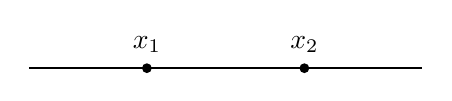
\begin{tikzpicture}
      \draw[thick, -] (0,0) -- (5,0);
      \node[circle,fill,inner sep=1.25pt,label=above:${x_1}$] (1) at (1.5,0) {};
      \node[circle,fill,inner sep=1.25pt,label=above:${x_2}$] (2) at (3.5,0) {};

    \end{tikzpicture}
  \end{center}
  Then there are 5 possible positions for $y_1$: we can have $y_1 = x_i$ for some $i$ or $y_1$ can
  lie on one of the lines, distinct from both $x_1$ and $x_2$. Then, since we need $y_1 < y_2$, the
  number of possible arrangements can be seen to be $5 + 5 + 3 + 3 + 1 = 13$. Including equality,
  we have 13 relation symbols, each representing a different ordering between the $x_i$ and $y_i$,
  which must mean that our relation symbols are exhaustive after all.

  Next we check that the relation symbols are mutually exclusive. This comes from the fact that each
  relation symbol encodes a separate possible ordering between the interval start and end points.
  As it is not possible to have 2 different orderings of the same fixed elements, the relation
  symbols must be mutually exclusive. For example, suppose that we have
  \begin{equation*}
    (x_1,x_2) \before (y_1,y_2) \qquad\qquad
    (x_1,x_2) \overlaps (y_1,y_2)
  \end{equation*}
  This happens only if we have both
  \begin{equation*}
    x_1 < x_2 < y_1 < y_2 \qquad\qquad
    x_1 < y_1 < x_2 < y_2
  \end{equation*}
  and so $x_2 < y_1 < x_2$. Since $<$ is irreflexive, this cannot happen.

  Checking transitivity is quite routine, the main difficulty being the sheer amount of cases. We
  will explicitly check the upper left quadrant in \cref{tab:transitivity} and leave the rest for
  the diligent reader. Fix $(x_1,x_2), (y_1,y_2), (z_1,z_2) \in \inter[L]$, which we will denote by
  $x,y,z$ respectively, then:
  \begin{itemize}
    \item Suppose that $x \before y$, so $x_1 < x_2 < y_1 < y_2$. If
      $y \aiaarrow{<mos} z$ then in all cases we must have
      $y_1 \leq z_1$, hence $x_1 < x_2 < z_1 < z_2$ and $x \before z$. On the other
      hand, if $y \aiaarrow{fd} z$ then we have $z_1 < y_1 \leq z_2$. This means
      that $x_2 < z_2$, restricting the possible relations between $x$ and $z$ to
      $x \aiaarrow{<mosd} z$ as expected.
    \item Suppose that $x \meets y$ so $x_1 < x_2 = y_1 < y_2$. If
      $y \aiaarrow{<mo} z$ then in all cases we must have $y_1 < z_1$ implying that
      $x \before z$. If $y \starts z$ then $y_1 = z_1 < z_2$ and
      $x \meets z$ too. Finally, if $y \aiaarrow{fd} z$ then we have
      $z_1 < y_1 < y_2 \leq z_2$, but $x_2 = y_1$ implying that $x \aiaarrow{osd} z$.
    \item Suppose that $x \overlaps y$, in which case we have $x_1 < y_1 < x_2 < y_2$. Then if
      $y \aiaarrow{<m} z$ we see that $x_1 < x_2 < z_1 < z_2$ so $x \before z$. If $y \overlaps z$
      then $x_1 < z_1$ and $x_2 < z_2$, leaving $x \aiaarrow{<mo} z$ as the only options. If
      $y \starts z$ then $x_1 < y_1 = z_1 < x_2 < y_2 < z_2$ so $x \overlaps z$ too. On the other
      hand if $y \aiaarrow{fd} z$ then $z_1 < x_2 < z_2$ and hence $x \aiaarrow{osd} z$.
    \item Suppose that $x \starts y$ so $x_1 = y_1 < x_2 < y_2$. In the case that $y \aiaarrow{<m} z$
      then $x_1 < x_2 < z_1 < z_2$, ie. $x \before z$. Similarly to before, if $y \overlaps z$ then
      $x_1<z_2$ and $x_2 < z_2$, so $x \aiaarrow{<mo} z$. If $y \starts z$ then we get
      $x_1 = y_1 = z_1 < x_2 < y_2 < z_2$ so $x \starts z$ too. For the last case, if
      $y \aiaarrow{fd} z$ then $z_1 < y_1 = x_1 < x_1 < y_2 \leq z_2$ so $x \contained z$.
    \item Suppose that $x \finishes y$, then $y_1 < x_1 < x_2 = y_2$. If $y \before z$ then we get
      $x_1 < x_2 = y_2 < z_1 < z_2$ and so $x \before z$. If $y \meets z$ then similarly we have
      $x_1 < x_2 = y_2 = z_1 < z_2$ so $x \meets z$.  In the case that $y \overlaps z$ we can see
      that $z_1 < y_2 = x_2 < z_2$ so $x \aiaarrow{osd} z$. If $x \aiaarrow{sd} z$ then
      $z_1 < y_1 = x_1 < x_2 < y_2 \leq z_2$, implying $x \contained z$. Finally, if $y \finishes z$
      then $z_1 < y_1 < x_1 < x_2 = y_2 = z_2$ and $x \finishes z$.
    \item Suppose that $x \contained y$ so $y_1 < x_1 < x_2 < y_2$. If $y \aiaarrow{<m} z$ then
      we have $x_1 < x_1 < y_2 \leq z_1 < z_2$ so $x \before z$. If $y \overlaps z$ then all we can
      say is that $x_2 < z_2$, leaving us with $x \aiaarrow{<mosd} z$. For the final case, if
      $y \aiaarrow{sfd} z$ then we end up with $z_1 \leq y_1 < x_1 < x_2 < y_2 \leq z_2$, so
      $x \contained z$.
  \end{itemize}
  The rest of the cases can be checked similarly.

  Finally, the different duality formulas hold by definition, so
  $\inter[L] \models \taia$.
\end{proof}

\begin{cor}
  Allen's interval algebras are satisfiable
\end{cor}

So the theory is satisfiable and it includes the main class of models we are interested in, models
coming from intervals over linear orders. Since the theory is relational and universal, it also
means that we can pick out any subset of intervals over a linear order and that will also give us a
model of $\taia$, which agrees with our intuition from the work Allen did originally. We will also
see later that every model of $\taia$ can be seen as a substructure of $\inter[L]$ for some linear
order $L$, which bodes well for our axiomatisation. But first, we need to develop some more
machinery.

Consider the function $\peq : \{0,1\}^2 \to \{ \laia-\text{formulas } \phi(I,J)\}$ defined by
\begin{align*}
  \peq(0,0)(I, J) & = (I \starts J) \lor (I \startedby J) \lor (I = J) \\
  \peq(0,1)(I, J) & = (I \metby J) \\
  \peq(1,0)(I, J) & = (I \meets J) \\
  \peq(1,1)(I, J) & = (I \finishes J) \lor (I \finishedby J) \lor (I = J)
\end{align*}
This function takes as inputs tuples $(n,m)$ with $n,m \in \{0,1\}$ and assigns them
the $\laia$-formulas $\peq(n,m)$ with $I$ and $J$ as free variables. We want to use this function
to quotient out the disjoint union $A + A$ in the following way:
\begin{equation*}
  (n,I) \psim (m,J) \iff A \models \peq(n,m)(I,J)
\end{equation*}
Of course, first we need to figure out whether this gives an equivalence relation.

\begin{prop}
  The relation $\psim$ defined as above is an equivalence relation on $A + A$.
\end{prop}
\begin{proof}
  The relation is reflexive, since $\peq(n,n)$ always contains $I = J$ as a disjunct, hence
  $A \models \peq(n,n)(I,I)$ and so $(n,I) \psim (n,I)$.

  The relation is also symmetric, since $A \models \peq(n,m)(I,J)$ if and only if
  $A \models \peq(m,n)(J,I)$. To see this, notice that the formula $\peq(m,n)$ is always given by
  taking the dual of the relation symbols in $\peq(n,m)$. Hence $(n,I) \psim (m,J)$ if and only if
  $(m,J) \psim (n,I)$.

  {\color{orange} TODO prove transitivity}
\end{proof}

\begin{defn}
  Given an Allen interval algebra $A$, we define the points of $A$ as
  \begin{equation*}
    \points[A] = \frac{A + A}{\psim}
  \end{equation*}
\end{defn}

Consider the function $\plt : \{0,1\}^2 \to \{ \laia-\text{formulas } \phi(I,J)\}$ defined by
\begin{align*}
  \plt(0,0)(I,J) & =(I \before J) \lor (I \meets J) \lor (I \overlaps J)
      \lor (I \finishedby J) \lor (I \contains J) \\
  \plt(0,1)(I,J) & = \lnot\,(I \after J) \land \lnot\,(I \metby J) \\
  \plt(1,0)(I,J) & = (I \before J) \\
  \plt(1,1)(I,J) & = (I \before J) \lor (I \meets J) \lor (I \overlaps J)
      \lor (I \starts J) \lor (I \contained J)
\end{align*}
Using this, we may order the start and end points of intervals in $A$, turning $\points[A]$ into
a strict linear order.

\begin{thm}
  Given an Allen interval algebra $A$, the interpretation of the symbol $<$ in $\points[A]$ given by
  $[(n,I)] < [(m,J)] \iff A \models \plt(n,m)(I,J)$ is well-defined and turns $A$ into a model of
  $\tslo$.
\end{thm}
\begin{proof}
  First we must check that this ordering relation on $\points[A]$ is well-defined. For this fix
  intervals $I_1,I_2,J_1,J_2 \in A$ and $n_1,n_2,m_1,m_2 \in \{0,1\}$ and assume that
  \begin{equation*}
    [(n_1,I_1)] = [(n_2,I_2)] < [(m_2,J_2)] = [(m_1,J_1)]
  \end{equation*}
  Then we must show that indeed, $[(n_1,I_1)] < [(m_1,J_1)]$. There are 16 distinct cases which
  we cover in \cref{tab:plt_well_defined}. Since, in each of the cases, with the possible relations
  $I_1 \longrightarrow J_1$ found in the last column, it is definitely the case that
  $A \models \plt(n_1,m_1)(I_1,J_1)$.

  \begin{table}[ht]
    \centering
    \setlength\extrarowheight{5pt}
    \begin{tabular}{|c|c|c|}
      \hline
      $(n_1,n_2,m_1,m_2)$ & Relation between $I_1,I_2,J_1,J_2$ & Relation between $I_1,J_1$ \\
      \hline\hline
      $(0,0,0,0)$ & $I_1 \aiaarrow{s=S} I_2 \aiaarrow{<moFD} J_2 \aiaarrow{s=S} I_1$ &
        $I_1 \aiaarrow{<moFD} J_1$ \\\hline
      $(0,0,0,1)$ & $I_1 \aiaarrow{s=S} I_2 \aiaarrow{<mosfd=OSFD} J_2 \aiaarrow{m} I_1$ &
        $I_1 \aiaarrow{<moFD} J_1$ \\\hline
      $(0,0,1,0)$ & $I_1 \aiaarrow{s=S} I_2 \aiaarrow{<moFD} J_2 \aiaarrow{M} I_1$ &
        $I_1 \aiaarrow{<mosfd=OSFD} J_1$ \\\hline
      $(0,0,1,1)$ & $I_1 \aiaarrow{s=S} I_2 \aiaarrow{<mosfd=OSFD} J_2 \aiaarrow{f=F} I_1$ &
        $I_1 \aiaarrow{<mosfd=OSFD} J_1$ \\\hline
      $(0,1,0,0)$ & $I_1 \aiaarrow{M} I_2 \aiaarrow{<} J_2 \aiaarrow{s=S} I_1$ &
        $I_1 \aiaarrow{<moFD} J_1 $ \\\hline
      $(0,1,0,1)$ & $I_1 \aiaarrow{M} I_2 \aiaarrow{<mosd} J_2 \aiaarrow{m} I_1$ &
        $I_1 \aiaarrow{<moFD} J_1 $ \\\hline
      $(0,1,1,0)$ & $I_1 \aiaarrow{M} I_2 \aiaarrow{<} J_2 \aiaarrow{M} I_1$ &
        $I_1 \aiaarrow{<mosfd=OSFD} J_1$ \\\hline
      $(0,1,1,1)$ & $I_1 \aiaarrow{M} I_2 \aiaarrow{<mosd} J_2 \aiaarrow{f=F} I_1$ &
        $I_1 \aiaarrow{<mosfd=OSFD} J_1$ \\\hline
      $(1,0,0,0)$ & $I_1 \aiaarrow{m} I_2 \aiaarrow{<moFD} J_2 \aiaarrow{s=S} I_1$ &
        $I_1 \aiaarrow{<} J_1$ \\\hline
      $(1,0,0,1)$ & $I_1 \aiaarrow{m} I_2 \aiaarrow{<mosfd=OSFD} J_2 \aiaarrow{m} I_1$ &
        $I_1 \aiaarrow{<} J_1$ \\\hline
      $(1,0,1,0)$ & $I_1 \aiaarrow{m} I_2 \aiaarrow{<moFD} J_2 \aiaarrow{M} I_1$ &
        $I_1 \aiaarrow{<mosd} J_1$ \\\hline
      $(1,0,1,1)$ & $I_1 \aiaarrow{m} I_2 \aiaarrow{<mosfd=OSFD} J_2 \aiaarrow{f=F} I_1$ &
        $I_1 \aiaarrow{<mosd} J_1$ \\\hline
      $(1,1,0,0)$ & $I_1 \aiaarrow{f=F} I_2 \aiaarrow{<} J_2 \aiaarrow{s=S} I_1$ &
        $I_1 \aiaarrow{<} J_1$ \\\hline
      $(1,1,0,1)$ & $I_1 \aiaarrow{f=F} I_2 \aiaarrow{<mosd} J_2 \aiaarrow{m} I_1$ &
        $I_1 \aiaarrow{<} J_1$ \\\hline
      $(1,1,1,0)$ & $I_1 \aiaarrow{f=F} I_2 \aiaarrow{<} J_2 \aiaarrow{M} I_1$ &
        $I_1 \aiaarrow{<mosd} J_1$ \\\hline
      $(1,1,1,1)$ & $I_1 \aiaarrow{f=F} I_2 \aiaarrow{<mosd} J_2 \aiaarrow{f=F} I_1$ &
        $I_1 \aiaarrow{<mosd} J_1$ \\\hline
    \end{tabular}
    \caption{
      All cases to check if the ordering on $\points[A]$ is well defined.
    }
    \label{tab:plt_well_defined}
  \end{table}

  Now we know that our definition of $<$ does not depend on a choice of representative, we need
  to check whether it satisfies $\tslo$:
  \begin{itemize}
    \item \textbf{irreflexivity}: Fix some element $[(n,I)] \in \points[A]$. Since the interval
      algebra relations (along with equality) are mutually exclusive and $I = I$, no other relation
      can hold for the pair $(I,I)$. Regardless of the value of $n$, $\plt(n,n)(I,I)$ does not
      include $I = I$ as a disjunct, so $A \not\models \plt(n,n)(I,I)$ and $<$ is irreflexive.
    \item \textbf{transitivity}: To show transitivity we start by fixing intervals $I,J,K \in A$ and
      assuming that $[(n,I)] < [(m,J)]$ and $[(m,J)] < [(l,K)]$. Then there are 8 cases
      based on the values of $n,m,k \in \{0,1\}$, all of which are considered in
      \cref{tab:plt_trans_000} up to \cref{tab:plt_trans_111}.
    \item \textbf{trichotomy}: Fix two $I,J \in A$. To check the trichotomy condition holds, we need
      to show that for all $n,m \in \{0,1\}$ we have
      \begin{equation*}
        A \models \plt(n,m)(I,J) \lor \peq(n,m)(I,J) \lor \plt(m,n)(J,I)
      \end{equation*}
      There are 3 cases that we must deal with separately to show this:
      \begin{itemize}
        \item First we consider $[(0,I)]$ and $[(0,J)]$. The formula $\plt(0,0)(I,J)$ is a
          disjunction 5 of our basic relations and $\plt(0,0)(J,I)$ the disjunction of its duals.
          Then $\peq(0,0)(I,J)$ is a disjunction of the 2 missing relations and equality. Hence by
          exhaustiveness of the interval algebra relations and equality, it must be the case that
          $A \models \plt(0,0)(I,J) \lor \peq(0,0)(I,J) \lor \plt(0,0)(J,I)$
        \item Next, we consider $[(0,I)]$ and $[(1,J)]$. Notice that the formula $\plt(0,1)(I,J)$
          is the negation of $\peq(0,1)(I,J) \lor \plt(1,0)(J,I)$, hence by the law of the
          excluded middle, the triple disjunction must hold.
        \item Finally we consider $[(1,I)]$ and $[(1,J)]$. The situation here is similar to the
          $n = m = 0$ case, since $\plt(1,1)(I,J)$ is a disjunction of 5 basic relations, then
          $\plt(1,1)(J,I)$ is the disjunction of its duals and $peq(1,1)(I,J)$ is the disjunction
          of the 2 missing relations plus equality.
      \end{itemize}
      When $(n,m)=(1,0)$, since $\psim$ is symmetric, we know that
      \begin{equation*}
        A \models \peq(1,0)(I,J) \iff A \models \peq(0,1)(J,I)
      \end{equation*}
      which allows us to reduce to the second case above.
  \end{itemize}
\end{proof}

In general, this will not be interpretable in the interval algebra $A$, since we need to
take the disjoint union of two sets which is not a priori available in first order logic.
However, provided that $|A| \neq 1$, then it is possible to define quotient $A^2$ by an appropriate
definable equivalence relation, something along the lines of
\begin{equation*}
  \phi(I,J) = \lnot (I = J)
\end{equation*}
So then we would encode $(0,I) \in A + A$ as the pair $(I,I) \in A^2$ and $(1,I) \in A + A$ as
$(I,J) \in A^2$ where $J$ is any interval different from $I$. Modifying the above definitions to
use this encoding would then show that the strict linear order $\inter[A]$ can be interpreted in
$A$.

% 0 0 0 case
\begin{table}[ht]
  \centering
  % \begin{tabular}{|c|c *{5}{|m{1.5cm}} |}
  %   \cline{3-7}
  %   \multicolumn{2}{c|}{} & \multicolumn{5}{c|}{$J \longrightarrow K$} \\\cline{3-7}
  %   \multicolumn{2}{c|}{} & < & m & o & F & D \\\hline
  %   \multirow{5}{*}{\begin{sideways}$I \longrightarrow J$\end{sideways}}
  %     & < & <     & <   & <   & <   & <     \\\cline{2-7}
  %     & m & <     & <   & <   & <   & <     \\\cline{2-7}
  %     & o & <     & <   & <mo & <mo & <moFD \\\cline{2-7}
  %     & F & <     & m   & o   & F   & D     \\\cline{2-7}
  %     & D & <moFD & oFD & oFD & D   & D     \\\hline
  %   \end{tabular}
  \begin{tabular}{| c | c | c || c | c | c || c | c | c |}
    \hline
    $I \to J$ & $J \to K$ & $I \to K$ &
      $I \to J$ & $J \to K$ & $I \to K$ &
      $I \to J$ & $J \to K$ & $I \to K$ \\
    \hline\hline
    \llrow & \olrow & \Dlrow \\
    \lmrow & \omrow & \Dmrow \\
    \lorow & \oorow & \Dorow \\
    \lFrow & \oFrow & \DFrow \\
    \lDrow & \oDrow & \DDrow \\
    \hline
    \mlrow & \Flrow &&&\\
    \mmrow & \Fmrow &&&\\
    \morow & \Forow &&&\\
    \mFrow & \FFrow &&&\\
    \mDrow & \FDrow &&&\\
    \hline
  \end{tabular}
  \caption{
    The transitivity table for the $[(0,I)] < [(0,J)]$ and $[(0,J)] < [(0,K)]$ case.
    For this to imply $[(0,I)] < [(0,K)]$ we need the $I \to K$ columns to all contain a
    subset of the string $<moFD$.
  }
  \label{tab:plt_trans_000}
\end{table}

% 0 0 1 case
\begin{table}[ht]
  \centering
  \begin{tabular}{| c | c | c || c | c | c || c | c | c |}
    \hline
    $I \to J$ & $J \to K$ & $I \to K$ &
      $I \to J$ & $J \to K$ & $I \to K$ &
      $I \to J$ & $J \to K$ & $I \to K$ \\
    \hline\hline
    \llrow & \olrow & \Dlrow \\
    \lmrow & \omrow & \Dmrow \\
    \lorow & \oorow & \Dorow \\
    \lsrow & \osrow & \Dsrow \\
    \lfrow & \ofrow & \Dfrow \\
    \ldrow & \odrow & \Ddrow \\
    \lerow & \oerow & \Derow \\
    \lOrow & \oOrow & \DOrow \\
    \lSrow & \oSrow & \DSrow \\
    \lFrow & \oFrow & \DFrow \\
    \lDrow & \oDrow & \DDrow \\
    \hline
    \mlrow & \Flrow &&&\\
    \mmrow & \Fmrow &&&\\
    \morow & \Forow &&&\\
    \msrow & \Fsrow &&&\\
    \mfrow & \Ffrow &&&\\
    \mdrow & \Fdrow &&&\\
    \merow & \Ferow &&&\\
    \mOrow & \FOrow &&&\\
    \mSrow & \FSrow &&&\\
    \mFrow & \FFrow &&&\\
    \mDrow & \FDrow &&&\\
    \hline
  \end{tabular}
  \caption{
    The transitivity table for the $[(0,I)] < [(0,J)]$ and $[(0,J)] < [(1,K)]$ case.
    For this to imply $[(0,I)] < [(1,K)]$ we need the $I \to K$ columns to all contain a
    subset of the string $<mosfd=OSFD$. Recall that concur is shorthand for $osfd=OSFD$
  }
  \label{tab:plt_trans_001}
\end{table}


% 0 1 0 case
\begin{table}[ht]
  \centering
  \begin{tabular}{| c | c | c |}
    \hline
    $I \to J$ & $J \to K$ & $I \to K$ \\
    \hline\hline
    \llrow \\
    \mlrow \\
    \olrow \\
    \slrow \\
    \flrow \\
    \dlrow \\
    \elrow \\
    \Olrow \\
    \Slrow \\
    \Flrow \\
    \Dlrow \\
    \hline
  \end{tabular}
  \caption{
    The transitivity table for the $[(0,I)] < [(1,J)]$ and $[(1,J)] < [(0,K)]$ case.
    For this to imply $[(0,I)] < [(0,K)]$ we need the $I \to K$ columns to all contain a
    subset of the string $<mofD$.
  }
  \label{tab:plt_trans_010}
\end{table}

% 0 1 1 case
\begin{table}[ht]
  \centering
  \begin{tabular}{| c | c | c || c | c | c || c | c | c |}
    \hline
    $I \to J$ & $J \to K$ & $I \to K$ &
      $I \to J$ & $J \to K$ & $I \to K$ &
      $I \to J$ & $J \to K$ & $I \to K$ \\
    \hline\hline
    \llrow & \flrow & \Slrow \\
    \lmrow & \fmrow & \Smrow \\
    \lorow & \forow & \Sorow \\
    \lsrow & \fsrow & \Ssrow \\
    \ldrow & \fdrow & \Sdrow \\
    \hline
    \mlrow & \dlrow & \Flrow \\
    \mmrow & \dmrow & \Fmrow \\
    \morow & \dorow & \Forow \\
    \msrow & \dsrow & \Fsrow \\
    \mdrow & \ddrow & \Fdrow \\
    \hline
    \olrow & \elrow & \Dlrow \\
    \omrow & \emrow & \Dmrow \\
    \oorow & \eorow & \Dorow \\
    \osrow & \esrow & \Dsrow \\
    \odrow & \edrow & \Ddrow \\
    \hline
    \slrow & \Olrow &&&\\
    \smrow & \Omrow &&&\\
    \sorow & \Oorow &&&\\
    \ssrow & \Osrow &&&\\
    \sdrow & \Odrow &&&\\
    \hline
  \end{tabular}
  \caption{
    The transitivity table for the $[(0,I)] < [(1,J)]$ and $[(1,J)] < [(1,K)]$ case.
    For this to imply $[(0,I)] < [(1,K)]$ we need the $I \to K$ columns to all contain a
    subset of the string $<mosfd=OSFD$. Recall that concur is shorthand for $osfd=OSFD$.
  }
  \label{tab:plt_trans_011}
\end{table}

% 1 0 0 case
\begin{table}[ht]
  \centering
  \begin{tabular}{| c | c | c |}
    \hline
    $I \to J$ & $J \to K$ & $I \to K$ \\
    \hline\hline
    \llrow \\
    \lmrow \\
    \lorow \\
    \lFrow \\
    \lDrow \\
    \hline
  \end{tabular}
  \caption{
    The transitivity table for the $[(1,I)] < [(0,J)]$ and $[(0,J)] < [(0,K)]$ case.
    For this to imply $[(1,I)] < [(0,K)]$ we need the $I \to K$ columns to all contain $<$.
  }
  \label{tab:plt_trans_100}
\end{table}

% 1 0 1 case
\begin{table}[ht]
  \centering
  \begin{tabular}{| c | c | c |}
    \hline
    $I \to J$ & $J \to K$ & $I \to K$ \\
    \hline\hline
    \llrow \\
    \lmrow \\
    \lorow \\
    \lsrow \\
    \lfrow \\
    \ldrow \\
    \lerow \\
    \lOrow \\
    \lSrow \\
    \lFrow \\
    \lDrow \\
    \hline
  \end{tabular}
  \caption{
    The transitivity table for the $[(1,I)] < [(0,J)]$ and $[(0,J)] < [(1,K)]$ case.
    For this to imply $[(1,I)] < [(1,K)]$ we need the $I \to K$ columns to all contain a
    subset of the string $<mosd$.
  }
  \label{tab:plt_trans_101}
\end{table}

% 1 1 0 case
\begin{table}[ht]
  \centering
  \begin{tabular}{| c | c | c |}
    \hline
    $I \to J$ & $J \to K$ & $I \to K$ \\
    \hline\hline
    \llrow \\
    \mlrow \\
    \olrow \\
    \slrow \\
    \dlrow \\
    \hline
  \end{tabular}
  \caption{
    The transitivity table for the $[(1,I)] < [(1,J)]$ and $[(1,J)] < [(0,K)]$ case.
    For this to imply $[(1,I)] < [(0,K)]$ we need the $I \to K$ columns to all contain $<$.
  }
  \label{tab:plt_trans_110}
\end{table}

% 1 1 1 case
\begin{table}[ht]
  \centering
  \begin{tabular}{| c | c | c || c | c | c || c | c | c |}
    \hline
    $I \to J$ & $J \to K$ & $I \to K$ &
      $I \to J$ & $J \to K$ & $I \to K$ &
      $I \to J$ & $J \to K$ & $I \to K$ \\
    \hline\hline
    \llrow & \olrow & \dlrow \\
    \lmrow & \omrow & \dmrow \\
    \lorow & \oorow & \dorow \\
    \lsrow & \osrow & \dsrow \\
    \ldrow & \odrow & \ddrow \\
    \hline
    \mlrow & \slrow &&&\\
    \mmrow & \smrow &&&\\
    \morow & \sorow &&&\\
    \msrow & \ssrow &&&\\
    \mdrow & \sdrow &&&\\
    \hline
  \end{tabular}
  \caption{
    The transitivity table for the $[(1,I)] < [(1,J)]$ and $[(1,J)] < [(1,K)]$ case.
    For this to imply $[(1,I)] < [(1,K)]$ we need the $I \to K$ columns to all contain a
    subset of the string $<mosd$.
  }
  \label{tab:plt_trans_111}
\end{table}

\newpage
\section{The Points-Intervals Adjunction}
\label{sec:adjunction}

\begin{defn}
  Given a theory $\theory$ over language $\lang$, we denote by $\mods{\lang}{\theory}$ the category
  with objects the models of $\theory$ and arrows the $\lang$-embeddings.
\end{defn}

\begin{rem}
  For brevity, we introduce the notation:
  \begin{equation*}
    \slos := \mods{\lslo}{\tslo} \text{ and } \aias := \mods{\laia}{\taia}
  \end{equation*}
\end{rem}

\begin{thm}
  We can turn $\inter$ into a functor
  \begin{equation*}
    \inter : \slos \to \aias
  \end{equation*}
  by sending arrows $f : M \to N$ in $\slos$ to  $\inter[f] : \inter[M] \to \inter[N]$ defined by
  \begin{equation*}
    \inter[f](x_1, x_2) = (f(x_1), f(x_2))
  \end{equation*}
\end{thm}
\begin{proof}
  First we show that for a $\lslo$-embedding $f : L \to M$ between strict linear orders
  $L,M$, the mapping $\inter[f]$ gives a an $\laia$-embedding. Consider the relations in $\laia$,
  and their interpretations in $\inter[L]$: all of the relations are defined by quantifier-free
  $\lslo$-formulas, whose truth value must be preserved under $\lslo$ embeddings like $f$. Since
  $\inter[f]$ simply applies $f$ pointwise, $\inter[f]$ must preserve the truth value of the
  relation symbols in $\laia$, in other words, it is an $\laia$-embedding.

  Now we just need to check that $\inter$ satisfies the two functor axioms:
  \begin{itemize}
    \item \textbf{preserves identity arrows}: Fix some strict linear order $L$ and some interval
      $(x,y) \in \inter[L]$, then
      \begin{equation*}
        \inter[\id{L}](x,y) = (\id{L}(x), \id{L}(y)) = (x,y)
      \end{equation*}
    \item \textbf{respects arrow composition}: Fix three strict linear orders $L,M,N$ along with
      arrows $f : L \to M$, $g : M \to N$ and some interval $(x,y) \in \inter[L]$, then
      \begin{align*}
        \inter[g \circ f](x,y)
          & = (g \circ f(x), g \circ f(y)) \\
          & = (g(f(x)), g(f(y))) \\
          & = \inter[g](\inter[f](x,y)) \\
          & = \inter[g]\circ\inter[f](x,y)
      \end{align*}
  \end{itemize}
\end{proof}

\begin{thm}
  We can turn $\points$ into a functor
  \begin{equation*}
    \points : \aias \to \slos
  \end{equation*}
  by sending arrows $f : A \to B$ in $\aias$ to $\points[f] : \points[A] \to \points[B]$
  defined by
  \begin{equation*}
    \points[f](0, I) = (0, f(I)) \qquad\text{and}\qquad \points[f](1,I) = (1, f(I))
  \end{equation*}
\end{thm}
\begin{proof}
  Given an arrow $f : A \to B$, we must check that $\points[f]$ is a well defined map, and that it
  is an $\lslo$-embedding. These facts both follow by noticing that $f$ is an
  $\laia$-embedding, so it preserves the truth of quantifier-free $\laia$-formulas, so
  \begin{align*}
    (n,I) \psim (m,J)
      & \iff A \models \peq(n,m)(I,J) \\
      & \iff A \models \peq(n,m)(f(I),f(J)) \\
      & \iff (n,f(I)) \psim (m,f(J))
  \end{align*}
  and similarly
  \begin{align*}
    [(n,I)] < [(m,J)]
      & \iff A \models \plt(n,m)(I,J) \\
      & \iff A \models \plt(n,m)(f(I),f(J)) \\
      & \iff \points[f]([(n,I)]) < \points[f]([(m,J)])
  \end{align*}
  for any two $(n,I),(m,J) \in A + A$, since $\peq(n,m)$ and $\plt(n,m)$ are always quantifier-free.

  Next, to see that $\points$ satisfies the functor axioms:
  \begin{itemize}
    \item \textbf{preserves identity arrows}: Fix some interval algebra $A$ and some element
    $[(n, I)] \in \points[A]$. Then notice that
      \begin{equation*}
        \points[\id{A}]([(n,I)]) = [(n, \id{A}(I))] = [(n,I)] = \id{\points[A]}([(n,I)])
      \end{equation*}
      Hence $\points[\id{A}] = \id{\points[A]}$.
    \item \textbf{respects arrow composition}: Fix interval algebras $A,B,C$ along with arrows
      $f : A \to B$, $g : B \to C$. Then for all elements $[(n,I)] \in \points[A]$:
      \begin{align*}
        \points[g \circ f]([(n,I)])
          & = [(n,g \circ f (I))] \\
          & = [(n, g(f(I)))] \\
          & = \points[g]\left( \points[f]([n,I]) \right) \\
          & = \points[g] \circ \points[f] ([n,I])
      \end{align*}
      Hence $\points[g \circ f] = \points[g] \circ \points[f]$ as expected.
  \end{itemize}
\end{proof}

\begin{rem}
  From now on, given an interval algebra $A$ and interval $I \in A$, we will use
  $\istart{I} := [(0,I)]$ and $\iend{I} := [(1,I)]$ to refer to the respective elements of
  $\points[A]$.
\end{rem}

\begin{thm}
  $\points$ is left adjoint to $\inter$.
\end{thm}
\begin{proof}
  We prove this through the Hom-Set definition of an adjunction, so we wish to find an isomorphism
  $\slos(\points[A],L) \cong \aias(A,\inter[L])$ which is natural in both $A$ and $L$.

  We start by defining the forward map
  \begin{equation*}
    \phi_{A,L} : \slos(\points[A],L) \to \aias(A,\inter[L])
  \end{equation*}
  which sends an $\lslo$-embedding $f : \points[A] \to L$ to the $\laia$-embedding
  \begin{equation*}
    \phi_{A,L}(f) : A \to \inter[L] \quad\text{sending}\quad
      I \mapsto (f(\istart{I}), f(\iend{I}))
  \end{equation*}
  To see this is a $\laia$-embedding, recall that it suffices to consider the $\aiaarrow{i}$
  relations for $i \in \aiaindex$, so we fix two intervals $I,J \in A$ and then:
  \begin{equation*}
    \begin{split}
      I \before J
        & \iff   \iend{I}  <   \istart{J} \\
        & \iff f(\iend{I}) < f(\istart{J}) \\
        & \iff \phi_{A,L}(f)(I) \before \phi_{A,L}(f)(J) \\
      I \meets J
        & \iff   \iend{I}  =   \istart{J} \\
        & \iff f(\iend{I}) = f(\istart{J}) \\
        & \iff \phi_{A,L}(f)(I) \meets \phi_{A,L}(f)(J) \\
      I \overlaps J
        & \iff   \istart{I}  <   \istart{J}  <   \iend{I}  <   \iend{J} \\
        & \iff f(\istart{I}) < f(\istart{J}) < f(\iend{I}) < f(\iend{J}) \\
        & \iff \phi_{A,L}(f)(I) \overlaps \phi_{A,L}(f)(J)
      \end{split}
      \begin{split}
      I \starts J
        & \iff   \istart{I}  =   \istart{J}  <   \iend{I}  <   \iend{J} \\
        & \iff f(\istart{I}) = f(\istart{J}) < f(\iend{I}) < f(\iend{J}) \\
        & \iff \phi_{A,L}(f)(I) \starts \phi_{A,L}(f)(J) \\
      I \finishes J
        & \iff   \istart{J}  <   \istart{I}  <   \iend{I}  =   \iend{J} \\
        & \iff f(\istart{J}) < f(\istart{I}) < f(\iend{I}) = f(\iend{J}) \\
        & \iff \phi_{A,L}(f)(I) \finishes \phi_{A,L}(f)(J) \\
      I \contained J
        & \iff   \istart{J}  <   \istart{I}  <   \iend{I}  <   \iend{J} \\
        & \iff f(\istart{J}) < f(\istart{I}) < f(\iend{I}) < f(\iend{J}) \\
        & \iff \phi_{A,L}(f)(I) \contained \phi_{A,L}(f)(J)
    \end{split}
  \end{equation*}

  Next, we define the inverse map
  \begin{equation*}
    \psi_{A,L} : \aias(A,\inter[L]) \to \slos(\points[A],L)
  \end{equation*}
  which sends an $\laia$-embedding $g : A \to \inter[L]$ to the $\lslo$-embedding given by
  \begin{equation*}
    \psi_{A,L}(f) : \points[A] \to L \quad\text{sending}\quad (n, I) \mapsto
      \left(\letin{(x_0,x_1) := g(I)}{x_n}\right)
  \end{equation*}
  Now, we need to ensure these maps are well defined and that they are indeed $\lslo$-embeddings. To
  check that $\psi_{A,L}(f)$ is well defined, we fix intervals $I,J \in A$ and get three cases to
  consider. In all of these cases we suppose $f(I) = (a,b)$ and $f(J) = (c,d)$:
  \begin{itemize}
    \item If $(0,I) \psim (0,J)$ then we must have
      \begin{equation*}
        A \models (I \starts J) \lor (I \startedby J) \lor (I = J)
      \end{equation*}
      Since $f$ is an $\laia$-embedding, this means that
      \begin{equation*}
        \inter[L] \models (f(I) \starts f(J)) \lor (f(I) \startedby f(J)) \lor (f(I) = f(J))
      \end{equation*}
      Equivalently, the above says that $a = c$, so
      $\psi_{A,L}(f)(\istart{I}) = a = c = \psi_{A,L}(f)(\istart{J})$.
    \item If $(0,I) \psim (1,J)$ then the following is true
      \begin{equation*}
        A \models I \metby J
      \end{equation*}
      Which implies that
      \begin{equation*}
        \inter[L] \models f(I) \metby f(J)
      \end{equation*}
      And this happens exactly when $a = d$, meaning
      $\psi_{A,L}(f)(\istart{I}) = a = d = \psi_{A,L}(f)(\iend{J})$. By symmetry of our equivalence
      relation this also deals with the $(1,I) \psim (0,J)$ case.
    \item If $(1,I) \psim (1,J)$ then
      \begin{equation*}
        A \models (I \finishes J) \lor (I \finishedby J) \lor (I = J)
      \end{equation*}
      And so
      \begin{equation*}
        \points[L] \models (f(I) \finishes f(J)) \lor (f(I) \finishedby f(J)) \lor (f(I) = f(J))
      \end{equation*}
      This implies that $b = d$ so $\psi_{A,L}(f)(\iend{I}) = b = d = \psi_{A,L}(f)(\iend{J})$ as
      needed.
  \end{itemize}

  To show monotonicity of $\psi_{A,L}(f)$ we get 4 distinct cases. Assuming again that
  $f(I) = (a,b)$ and $f(J) = (c,d)$:
  \begin{itemize}
    \item If $\istart{I} < \istart{J}$ then we must have
      \begin{equation*}
        A \models (I \before J) \lor (I \meets J) \lor (I \overlaps J)  \lor (I \finishedby J)
                                \lor (I \contains J)
      \end{equation*}
      Since $f$ is an $\laia$-embedding, this means that
      \begin{align*}
        \inter[L] \models\, & (f(I) \before f(J)) \lor (f(I) \meets f(J)) \lor (f(I) \overlaps f(J)) \\
                            & \qquad \lor (f(I) \finishedby f(J)) \lor (f(I) \contains f(J))
      \end{align*}
      This means the ordering of the elements $a,b,c,d$ must be one of:
      \begin{gather*}
        a < b < c < d \qquad a < b = c = d  \qquad a < c < b < d \\
        a < c < d = b \qquad a < c < d < b
      \end{gather*}
      And in all cases $\psi_{A,L}(f)(\istart{I}) = a < c = \psi_{A,L}(f)(\istart{J})$.
    \item If $\istart{I} < \iend{J}$ then we must have
      \begin{equation*}
        A \models \lnot\,(I \after J) \land \lnot\,(I \metby J)
      \end{equation*}
      Since $f$ is an $\laia$-embedding, this means that
      \begin{equation*}
        \inter[L] \models \lnot\,(f(I) \after f(J)) \land \lnot\,(f(I) \metby f(J))
      \end{equation*}
      This is the case with the most orderings of $a,b,c,d$, having one of:
      \begin{gather*}
        a < b < c < d \qquad a < b = c < d \qquad a < c < b < d \qquad a = c < b < d \\
        c < a < b = d \qquad c < a < b < d \qquad a = c < b = d \qquad c < a < d < b \\
        a = c < d < b \qquad a < c < d = b \qquad a < c < d < b
      \end{gather*}
      In all cases though, $\psi_{A,L}(f)(\istart{I}) = a < d = \psi_{A,L}(f)(\iend{J})$.
    \item If $\iend{I} < \istart{J}$ then we must have
      \begin{equation*}
        A \models I \before J
      \end{equation*}
      Since $f$ is an $\laia$-embedding, this means that
      \begin{equation*}
        \inter[L] \models f(I) \before f(J)
      \end{equation*}
      So in $L$ we must have $a < b < c < d$, and so
      $\psi_{A,L}(f)(\iend{I}) = b < c = \psi_{A,L}(f)(\istart{J})$.
    \item If $\iend{I} < \iend{J}$ then we must have
      \begin{equation*}
        A \models (I \before J) \lor (I \meets J) \lor (I \overlaps J) \lor (I \starts J)
                                \lor (I \contained J)
      \end{equation*}
      Since $f$ is an $\laia$-embedding, this means that
      \begin{align*}
        \inter[L] \models\, & (f(I) \before f(J)) \lor (f(I) \meets f(J)) \lor (f(I) \overlaps f(J)) \\
                          & \qquad \lor (f(I) \starts f(J)) \lor (f(I) \contained f(J)
      \end{align*}
      This gives 5 possible orderings of $a,b,c,d$ in $L$:
      \begin{gather*}
        a < b < c < d \qquad a < b = c = d  \qquad a < c < b < d \\
        a = c < b < d \qquad c < a < b < d
      \end{gather*}
      As $b < d$ in all of these, the ordering is preserved by $\psi_{A,L}(f)$.
  \end{itemize}

  We expect $\phi_{A,L}$ and $\psi_{A,L}$ to be inverses, which is confirmed by the following:
  \begin{itemize}
    \item Pick  any $f : \points[A] \to L$ and $[(n,I)] \in \points[A]$, then
      \begin{align*}
        \psi_{A,L}\left(\phi_{A,L}(f)\right)([(n,I)])
          & = \left( \letin{(x_0,x_1) := \phi_{A,L}(f)(I)}{x_n} \right) \\
          & = \left( \letin{(x_0,x_1) := (f(\istart{I}), f(\iend{I}))}{x_n} \right) \\
          & = f([n, I])
      \end{align*}
    \item Pick any $g : A \to \inter[L]$ and $I \in A$, then
      \begin{equation*}
        \phi_{A,L}\left(\psi_{A,L}(g)\right)(I)
          = \left( \psi_{A,L}(g)(\istart{I}), \psi_{A,L}(g)(\iend{I}) \right)
          = g(I)
      \end{equation*}
  \end{itemize}

  Finally, we just have to check naturality of our isomorphism $\phi_{A,L}$. So pick a
  $\laia$-embedding $f : A \to B$ and a $\lslo$-embeddings $g : L \to M$, we need to show the
  following diagram commutes
  % If modifying diagram, don't forget to add [scale cd=0.99]
  % https://q.uiver.app/?q=WzAsNixbMywwLCJcXHNsb3MoXFxwb2ludHNbQV0sTCkiXSxbMywyLCJcXGFpYXMoQSxcXGludGVyW0xdKSJdLFswLDAsIlxcc2xvcyhcXHBvaW50c1tCXSxMKSJdLFswLDIsIlxcYWlhcyhCLFxcaW50ZXJbTF0pIl0sWzYsMiwiXFxhaWFzKEEsXFxpbnRlcltNXSkiXSxbNiwwLCJcXHNsb3MoXFxwb2ludHNbQV0sTSkiXSxbMiwwLCJcXHNsb3MoXFxwb2ludHNbZl0sTCkiXSxbMywxLCJcXGFpYXMoZixcXGludGVyW0xdKSIsMl0sWzIsMywiXFxwaGlfe0IsTH0iLDJdLFsxLDQsIlxcYWlhcyhBLFxcaW50ZXJbZ10pIiwyXSxbMCw1LCJcXHNsb3MoXFxwb2ludHNbQV0sZykiXSxbNSw0LCJcXHBoaV97QSxNfSJdLFswLDEsIlxccGhpX3tBLEx9IiwyXV0=
  \[\begin{tikzcd}[scale cd=0.99]
    {\slos(\points[B],L)} &&& {\slos(\points[A],L)} &&& {\slos(\points[A],M)} \\
    \\
    {\aias(B,\inter[L])} &&& {\aias(A,\inter[L])} &&& {\aias(A,\inter[M])}
    \arrow["{\slos(\points[f],L)}", from=1-1, to=1-4]
    \arrow["{\aias(f,\inter[L])}"', from=3-1, to=3-4]
    \arrow["{\phi_{B,L}}"', from=1-1, to=3-1]
    \arrow["{\aias(A,\inter[g])}"', from=3-4, to=3-7]
    \arrow["{\slos(\points[A],g)}", from=1-4, to=1-7]
    \arrow["{\phi_{A,M}}", from=1-7, to=3-7]
    \arrow["{\phi_{A,L}}"', from=1-4, to=3-4]
  \end{tikzcd}\]
  We do this by checking both squares individually:
  \begin{itemize}
    \item \textbf{left square}: Pick some $h : \slos(\points[B],L)$ and $I \in A$, then
      \begin{align*}
        \phi_{A,L}(\slos(\points[f],L)(h))(I)
          & = \phi_{A,L}(h \circ \points[f])(I) \\
          & = (h(\points[f](\istart{I})), h(\points[f](\iend{I}))) \\
          & = (h(\istart{f(I)}), h(\iend{f(I)})) \\
          & = \phi_{B,L}(h)(f(I)) \\
          & = \phi_{B,L}(h) \circ f(I) \\
          & = \aias(f,\inter[L])(\phi_{B,L}(h))(I)
      \end{align*}
    \item \textbf{right square}: Pick some $h : \slos(\points[A],L)$ and $I \in A$, then
      \begin{align*}
        \phi_{A,M}(\slos(\points[A],g)(h))(I)
          & = \phi_{A,M}(g \circ h)(I) \\
          & = (g(h(\istart{I})), g(h(\iend{I}))) \\
          & = (g(h(\istart{I})), g(h(\iend{I}))) \\
          & = \inter[g](h(\istart{I}), h(\iend{I})) \\
          & = \inter[g](\phi_{A,L}(h)(I)) \\
          & = \aias(A,\inter[g])(\phi{A,L}(h))(I)
      \end{align*}
  \end{itemize}

  % For an interval algebra $A$ and a strict linear order $L$, we have
  % \begin{equation*}
  %   \text{Hom}(\points[A], L) \cong \text{Hom}(A, \inter[L])
  % \end{equation*}
  % A map of linear orders from the start/end points of A to L, enforces a mapping of interval
  % algebras from A to the intervals of L, by checking where the start/end points of the interval end.

  % The above map is "canonical" so it should be natural in A and L.
\end{proof}

In order to get a bit more familiar with these constructions, it can be beneficial to see why
$\points$ is not right  adjoint to $\inter$, that is, in general
we do not have that
\begin{equation*}
  \aias(\inter[L],A) \cong \slos(L,\points[A])
\end{equation*}
for all strict linear orders $L$
and interval algebras $A$. For example, consider the interval algebra $A$ given by the set
$A = \{I, J, K\}$ with the relations between intervals $I \overlaps J, J \meets K, I \before K$.
Applying the $\points$ construction to $A$ gives a linear order with 5 elements, as can be seen in
\cref{fig:points_example}. We will also need the linear order $L = \{1 < 2 < 3\}$, which
has 3 intervals, as seen in \cref{fig:inter_example}. Now, an order preserving embedding
$f : L \to \points[A]$ simply needs to pick 3 distinct points in $\points[A]$. There are
$\binom{5}{3} = 10$ possible ways of picking 3 distinct points out of $\points[A]$, so we see
that $|\slos(L,\points[A])| = 10$. On the other hand, an embedding of interval algebras
$f : \inter[L] \to A$ must pick out two intervals in $A$ which meet (the images of $(1,2)$ and
$(2,3)$) with the constraint that the "union" of these two intervals exists in $A$. In this specific
case, our only option is that $f((1,2)) = J$ and $f((2,3)) = K$, but there is no interval which
is started by $J$ and finished by $K$, so there is nowhere to map $(1,3)$ to. This means that
$\aias(\inter[L],A) = \emptyset$, so there can be no isomorphism between this and
$\slos(L,\points[A])$.


\begin{figure}[ht]
  \centering
  \begin{tikzpicture}
    \draw[dashed, color=gray, -] (0,0)     -- (0, -3);
    \draw[dashed, color=gray, -] (3,0)     -- (3, -3);
    \draw[dashed, color=gray, -] (2,-0.75) -- (2, -3);
    \draw[dashed, color=gray, -] (6,-0.75) -- (6, -3);
    \draw[dashed, color=gray, -] (10,-1.5) -- (10, -3);

    \draw[thick, |-|] (0,0)     -- (3,0)     node[above, midway] {$I$};
    \draw[thick, |-|] (2,-0.75) -- (6,-0.75) node[above, midway] {$J$};
    \draw[thick, |-|] (6,-1.5)  -- (10,-1.5) node[above, midway] {$K$};

    \draw[thin, -] (0,-3) -- (10,-3);
    \node[circle,fill,inner sep=1.25pt,label=below:$\istart{I}$]            (1) at (0, -3) {};
    \node[circle,fill,inner sep=1.25pt,label=below:$\istart{J}$]            (2) at (2, -3) {};
    \node[circle,fill,inner sep=1.25pt,label=below:$\iend{I}$]              (3) at (3, -3) {};
    \node[circle,fill,inner sep=1.25pt,label=below:{$\iend{J}=\istart{K}$}] (4) at (6, -3) {};
    \node[circle,fill,inner sep=1.25pt,label=below:$\iend{K}$]              (5) at (10, -3) {};

    \node (A)       at (-2, -0.75) {$A$};
    \node (pointsA) at (-2, -3)    {$\points[A]$};
    \draw [very thick,decorate,decoration = {brace}] (-1,-1.6) -- (-1,0.1);
    \draw [very thick,decorate,decoration = {brace}] (-1,-3.3) -- (-1,-2.7);
  \end{tikzpicture}
  \caption{An example of the $\points$ construction.}
  \label{fig:points_example}
\end{figure}

\begin{figure}[ht]
  \centering
  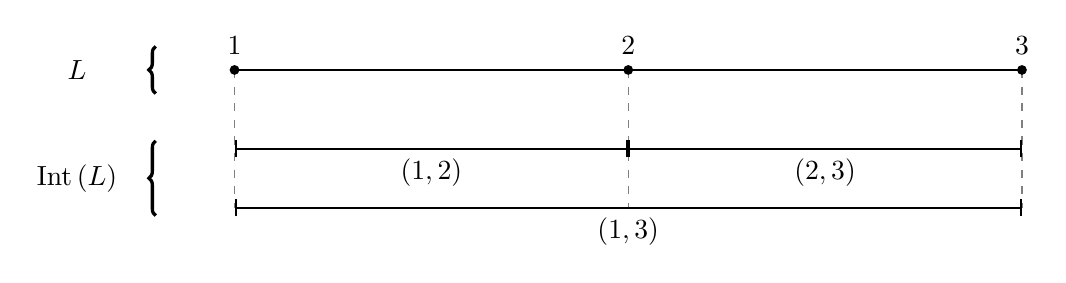
\begin{tikzpicture}
    \draw[dashed, color=gray, -] (0,0) -- (0, -1.75);
    \draw[dashed, color=gray, -] (5,0) -- (5, -1.75);
    \draw[dashed, color=gray, -] (10,0) -- (10, -1.75);

    \draw [thin,-] (0,0) -- (10,0);
    \node[circle,fill,inner sep=1.25pt,label=above:$1$] (1) at (0,0)  {};
    \node[circle,fill,inner sep=1.25pt,label=above:$2$] (2) at (5,0)  {};
    \node[circle,fill,inner sep=1.25pt,label=above:$3$] (3) at (10,0) {};

    \draw[thick, |-|] (0,-1) -- (5,-1) node[below, midway] {$(1,2)$};
    \draw[thick, |-|] (5,-1) -- (10,-1) node[below, midway] {$(2,3)$};
    \draw[thick, |-|] (0,-1.75) -- (10,-1.75) node[below, midway] {$(1,3)$};

    \node (L)      at (-2, 0)     {$L$};
    \node (interL) at (-2, -1.375) {$\inter[L]$};
    \draw [very thick,decorate,decoration = {brace}] (-1,-0.3) -- (-1,0.3);
    \draw [very thick,decorate,decoration = {brace}] (-1,-1.85) -- (-1,-0.9);
  \end{tikzpicture}
  \caption{An example of the $\inter$ construction}
  \label{fig:inter_example}
\end{figure}

\subsection{Characterising the Unit and Counit}%
\label{sub:characterising_the_unit_and_counit}

Given an adjunction, it is always helpful to compute the associated unit and counit natural
transformations. In our case, the unit is a natural transformation
$\unit{} : \id{\aias} \to \inter[\points]$
whose component at an interval algebra $A$ is given by
$\unit{A} = \phi_{A,\points[A]}(\id{\points[A]})$. Computing this, we get the map
\begin{equation*}
  \unit{A} : A \to \inter[\points[A]] \text{ sending } I \mapsto (\istart{I}, \iend{I})
\end{equation*}
Recall that each component of the unit $\unit{A}$ is an arrow in $\aias$, so it must be an
embedding. This means that every interval algebra $A$ can be seen as a substructure of the intervals
$\inter[L]$ for some appropriate linear order, namely $L = \points[A]$.

Dually, the counit here is a natural transformation $\counit{} : \points[\inter] \to \id{\slos}$
where each of its components is given by $\counit{L} = \psi_{\inter[L],L}(\id{\inter[L]})$.
Fixing some $L$ and working through this construction, we get
\begin{equation*}
  \counit{L} : \points[\inter[L]] \to L \text{ sending }
    \istart{(a,b)} \mapsto a \text{ and } \iend{(a,b)} \mapsto b
\end{equation*}

\begin{prop}
The counit component at a strict linear order $L$, $\counit{L}$, is an isomorphism if and only if
$|L| \neq 1$.
\end{prop}
\begin{proof}
  First, suppose that $|L|=1$, so $L = \{a\}$. Then $\inter[L] = \emptyset$ as we do not allow empty
  intervals and so $\points[\inter[L]] = \emptyset$ too. As such, $\counit{L}$ cannot be an
  isomorphism.

  For the converse, notice that $\counit{L}$ is a map in $\slos$, hence it must be injective.
  Provided that $|L| \neq 1$ then it also turns out to be surjective: fix some
  $a \in L$, there must be at least one distinct $b \in L$. Now either $a < b$, so $(a,b)$ is a
  valid interval over $L$ and then $\counit{L}(\istart{(a,b)}) = a$. Alternatively, $b < a$, so
  $(b, a)$ is an interval in $\inter[L]$ and $\counit{L}(\iend{(b,a)}) = a$
\end{proof}

As for the unit, it will give us an isomorphism when our interval algebra already has all possible
intervals. More precisely, we will say that an interval algebra has all possible intervals if it
satisfies the following sentence
\begin{align*}
  \allints = & \left(\forall I,\; \forall J,\;
        (I \before J)    \rightarrow \exists K,\; (I \meets K)      \land (K \meets J)    \right)\\
    & \land \left(\forall I,\; \forall J,\;
        (I \meets J)     \rightarrow \exists K,\; (I \startedby K)  \land (K \finishes J) \right)\\
    & \land \left(\forall I,\; \forall J,\;
        (I \overlaps J)  \rightarrow \exists K,\; (I \finishedby K) \land (K \starts J)   \right)\\
    & \land \left(\forall I,\; \forall J,\;
        (I \starts J)    \rightarrow \exists K,\; (I \meets K)      \land (K \finishes J) \right)\\
    & \land \left(\forall I,\; \forall J,\;
        (I \finishes J)  \rightarrow \exists K,\; (I \metby K)      \land (K \starts J)   \right)\\
    & \land \left(\forall I,\; \forall J,\;
        (I \contained J) \rightarrow \exists K,\; (I \metby K)      \land (K \starts J)   \right)
\end{align*}

The above formula does not specify it, but it can be shown that the $K$ being quantified over
must actually be unique. For example, fix some $I$ and $J$ such that $I \before J$ and let there
be two $K_1,K_2$ such that $I \meets K_i \meets J$. Then we have $K_1 \metby I \meets K_2$, implying
that $K_1 \aiaarrow{s=S} K_2$. If $K_1 \starts K_2$ then $K_1 \starts K_2 \meets J$ and our axioms
mean that $K_1 \before J$, which is a contradiction as the interval algebra relations are mutually
exclusive. Similarly we can show that $K_1 \startedby K_2$ cannot happen, leaving us with
the only option of $K_1 = K_2$. Similar arguments show the uniqueness of $K$ in the other cases.

\begin{prop}
  The unit component at an interval algebra $A$, $\unit{A}$, is an isomorphism if and only if
  $A \models \allints$.
\end{prop}
\begin{proof}
  First, suppose that $\unit{A}$ is an isomorphism. To show that $A \models allints$ we fix
  two intervals $I,J \in A$. Now we have to consider 6 cases:
  \begin{itemize}
    \item If $I \before J$ then in $\inter[\points[A]]$ we must have
      $\istart{I} < \iend{I} < \istart{J} < \iend{J}$. This means the following are all valid
      intervals
      \begin{equation*}
        \unit{A}(I) = (\istart{I}, \iend{I}) \meets (\iend{I}, \istart{J})
          \meets (\istart{J}, \iend{J}) = \unit{A}(J)
      \end{equation*}
      so taking $K = \unit{A}^{-1}((\iend{I},\istart{J}))$ we see that the first conjunct holds.
    \item If $I \meets J$ then $\istart{I} < \iend{I} = \istart{J} < \iend{J}$, hence taking
      $K = \unit{A}^{-1}((\istart{I}, \iend{J}))$ shows that the second conjunct holds.
    \item If $I \overlaps J$ then $\istart{I} < \istart{J} < \iend{I} < \iend{J}$ and we can take
      $K = \unit{A}^{-1}((\istart{J}, \iend{I}))$ to prove the third conjunct.
    \item If $I \starts J$ then $\istart{I} = \istart{J} < \iend{I} < \iend{J}$, so taking
      $K = \unit{A}^{-1}((\iend{I}, \iend{J}))$ proves the fourth conjunct.
    \item If $I \finishes J$ then $\istart{J} < \istart{I} < \iend{I} = \iend{J}$ so the choice
      $K = \unit{A}^{-1}((\istart{J}, \istart{I}))$ gives a proof of the penultimate conjunct.
    \item If $I \contained J$ then $\istart{J} < \istart{I} < \iend{I} < \iend{J}$ and if we let
      $K = \unit{A}^{-1}((\istart{J}, \istart{I}))$ then we see the last conjunct holds too.
  \end{itemize}
  As all conjuncts hold, this implies that $A \models \allints$ as expected.

  Next, suppose that we have an interval algebra $A$ such that $A \models \allints$ and fix two intervals
  $I,J \in A$. Since $I$ and $J$ are arbitrary, it will suffice to consider the basic non-dual
  relations.
  \begin{itemize}
    \item If $I \before J$ then we get some $K_1$ which is met by $I$ and meets $J$. Then we can glue
      $I$ and $K_1$ to get $K_2$ and similarly we glue $K_1$ and $J$ to get $K_3$. Finally, gluing
      $K_2$ and $J$ gives us $K_4$. This gives the following picture
      \begin{center}
        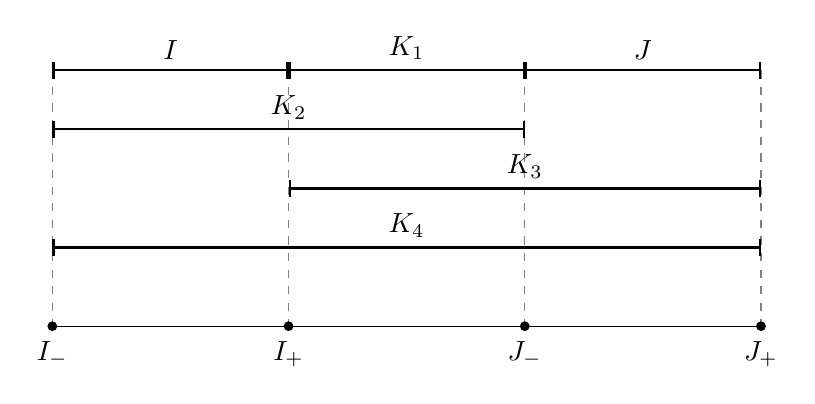
\begin{tikzpicture}
          \draw[dashed, color=gray, -] (0,0) -- (0, -3.25);
          \draw[dashed, color=gray, -] (3,0) -- (3, -3.25);
          \draw[dashed, color=gray, -] (6,0) -- (6, -3.25);
          \draw[dashed, color=gray, -] (9,0) -- (9, -3.25);

          \draw [thin,-] (0,-3.25) -- (9,-3.25);
          \node[circle,fill,inner sep=1.25pt,label=below:$\istart{I}$] (1) at (0,-3.25)  {};
          \node[circle,fill,inner sep=1.25pt,label=below:$\iend{I}$] (2) at (3,-3.25)  {};
          \node[circle,fill,inner sep=1.25pt,label=below:$\istart{J}$] (3) at (6,-3.25) {};
          \node[circle,fill,inner sep=1.25pt,label=below:$\iend{J}$] (3) at (9,-3.25) {};

          \draw[thick, |-|] (0,0) -- (3,0) node[above, midway] {$I$};
          \draw[thick, |-|] (6,0) -- (9,0) node[above, midway] {$J$};
          \draw[thick, |-|] (3,0)  -- (6,0) node[above, midway] {$K_1$};
          \draw[thick, |-|] (0,-0.75)  -- (6,-0.75) node[above, midway] {$K_2$};
          \draw[thick, |-|] (3,-1.5)  -- (9,-1.5) node[above, midway] {$K_3$};
          \draw[thick, |-|] (0,-2.25)  -- (9,-2.25) node[above, midway] {$K_4$};
        \end{tikzpicture}
      \end{center}
      Then the unit $\unit{A}$ surjects on all intervals over the start and end points of $I,J$:
      \begin{align*}
        (\istart{I},\istart{J}) = \unit{A}(K_2) \qquad\qquad (\istart{I},\iend{J}) = \unit{A}(K_4) \\
        (\iend{I},\istart{J}) = \unit{A}(K_1)   \qquad\qquad (\iend{I},\iend{J}) = \unit{A}(K_3)
      \end{align*}
    \item If $I \meets J$ then we can glue $I$ and $J$ to get $K$, yielding the following
      \begin{center}
        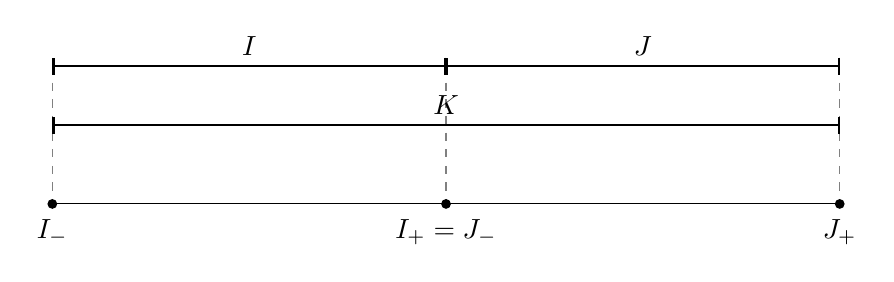
\begin{tikzpicture}
          \draw[dashed, color=gray, -] (0,0) -- (0, -1.75);
          \draw[dashed, color=gray, -] (5,0) -- (5, -1.75);
          \draw[dashed, color=gray, -] (10,0) -- (10, -1.75);

          \draw [thin,-] (0,-1.75) -- (10,-1.75);
          \node[circle,fill,inner sep=1.25pt,label=below:$\istart{I}$] (1) at (0,-1.75)  {};
          \node[circle,fill,inner sep=1.25pt,label=below:${\iend{I}=\istart{J}}$] (2) at (5,-1.75) {};
          \node[circle,fill,inner sep=1.25pt,label=below:$\iend{J}$] (3) at (10,-1.75) {};

          \draw[thick, |-|] (0,0) -- (5,0) node[above, midway] {$I$};
          \draw[thick, |-|] (5,0)  -- (10,0) node[above, midway] {$J$};
          \draw[thick, |-|] (0,-0.75) -- (10,-0.75) node[above, midway] {$K$};
        \end{tikzpicture}
      \end{center}
      The unit also surjects on all valid intervals over the start and end poits of $I,J$:
      \begin{align*}
        (\istart{I},\istart{J}) = \unit{A}(J)   \qquad (\istart{I},\iend{J}) = \unit{A}(K)
          \qquad (\iend{I},\iend{J}) = \unit{A}(J)
      \end{align*}
      In this case there are only 3 in this case since $\iend{I} = \istart{J}$ so
      $(\iend{I}, \istart{J})$ is not a valid interval over $\points[A]$.
    \item If $I \overlaps J$ then first we intersect $I$ and $J$ giving $K_1$. Similarly we can
      intersect $K_1$ with $I$ and $J$ giving $K_2$ and $K_3$ respectively. Finally gluing $I$ and
      $K_3$ together gives $K_4$.
      \begin{center}
        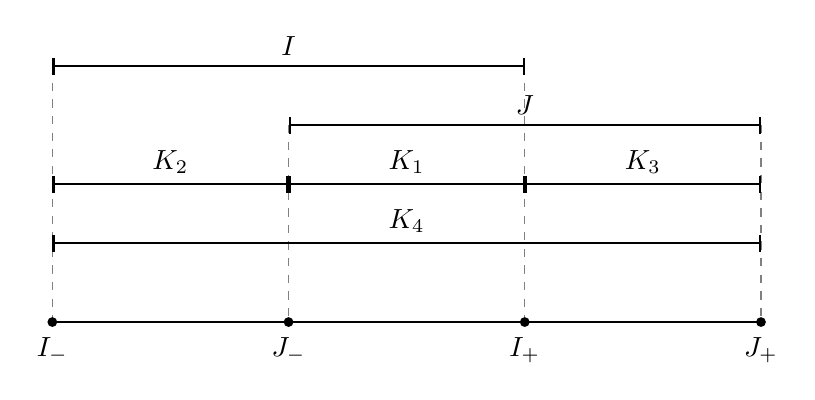
\begin{tikzpicture}
          \draw[dashed, color=gray, -] (0,0) -- (0, -3.25);
          \draw[dashed, color=gray, -] (3,-0.75) -- (3, -3.25);
          \draw[dashed, color=gray, -] (6,0) -- (6, -3.25);
          \draw[dashed, color=gray, -] (9,-0.75) -- (9, -3.25);

          \draw [thin,-] (0,-3.25) -- (9,-3.25);
          \node[circle,fill,inner sep=1.25pt,label=below:$\istart{I}$] (1) at (0,-3.25)  {};
          \node[circle,fill,inner sep=1.25pt,label=below:$\istart{J}$] (2) at (3,-3.25)  {};
          \node[circle,fill,inner sep=1.25pt,label=below:$\iend{I}$] (3) at (6,-3.25) {};
          \node[circle,fill,inner sep=1.25pt,label=below:$\iend{J}$] (3) at (9,-3.25) {};

          \draw[thick, |-|] (0,0) -- (6,0) node[above, midway] {$I$};
          \draw[thick, |-|] (3,-0.75) -- (9,-0.75) node[above, midway] {$J$};
          \draw[thick, |-|] (6,-1.5) -- (9,-1.5) node[above, midway] {$K_3$};
          \draw[thick, |-|] (0,-1.5) -- (3,-1.5) node[above, midway] {$K_2$};
          \draw[thick, |-|] (3,-1.5)  -- (6,-1.5) node[above, midway] {$K_1$};
          \draw[thick, |-|] (0,-2.25)  -- (9,-2.25) node[above, midway] {$K_4$};
        \end{tikzpicture}
      \end{center}
      Similar to the $I \before J$ case, the unit is then surjective onto the 4 possible intervals
      involving $\istart{I}, \iend{I}, \istart{J}, \iend{J}$.
    \item When $I \starts J$ we can intersec $I$ and $J$ to get $K$
      \begin{center}
        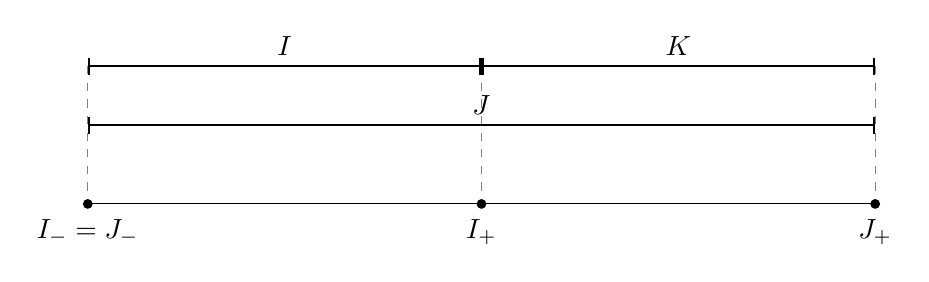
\begin{tikzpicture}
          \draw[dashed, color=gray, -] (0,0) -- (0, -1.75);
          \draw[dashed, color=gray, -] (5,0) -- (5, -1.75);
          \draw[dashed, color=gray, -] (10,0) -- (10, -1.75);

          \draw [thin,-] (0,-1.75) -- (10,-1.75);
          \node[circle,fill,inner sep=1.25pt,label=below:${\istart{I}=\istart{J}}$] (1) at (0,-1.75)  {};
          \node[circle,fill,inner sep=1.25pt,label=below:$\iend{I}$] (2) at (5,-1.75) {};
          \node[circle,fill,inner sep=1.25pt,label=below:$\iend{J}$] (3) at (10,-1.75) {};

          \draw[thick, |-|] (0,0) -- (5,0) node[above, midway] {$I$};
          \draw[thick, |-|] (0,-0.75) -- (10,-0.75) node[above, midway] {$J$};
          \draw[thick, |-|] (5,0)  -- (10,0) node[above, midway] {$K$};
        \end{tikzpicture}
      \end{center}
      We get 4 intervals over the start and end points of $I$ and $J$, which are given by
      \begin{align*}
        (\istart{I},\iend{J}) = \unit{A}(J) \qquad (\istart{I},\iend{I}) = \unit{A}(I)
          \qquad (\iend{I},\iend{J}) = \unit{A}(K)
      \end{align*}
    \item The $I \finishes J$ follows similarly to the previous case, by intersecting $I$ and $J$ to
      get $K$
      \begin{center}
        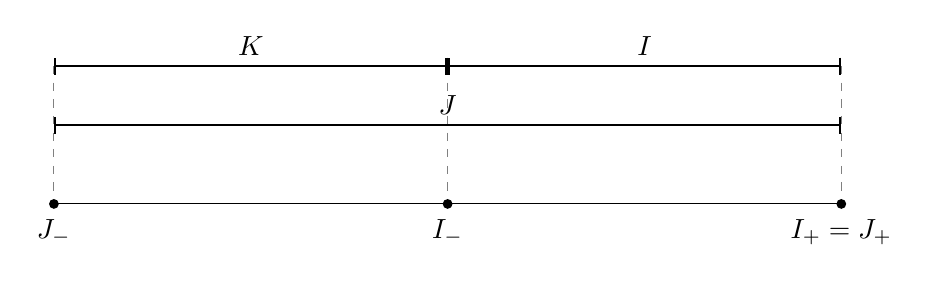
\begin{tikzpicture}
          \draw[dashed, color=gray, -] (0,0) -- (0, -1.75);
          \draw[dashed, color=gray, -] (5,0) -- (5, -1.75);
          \draw[dashed, color=gray, -] (10,0) -- (10, -1.75);

          \draw [thin,-] (0,-1.75) -- (10,-1.75);
          \node[circle,fill,inner sep=1.25pt,label=below:$\istart{J}$] (1) at (0,-1.75)  {};
          \node[circle,fill,inner sep=1.25pt,label=below:$\istart{I}$] (2) at (5,-1.75) {};
          \node[circle,fill,inner sep=1.25pt,label=below:${\iend{I} = \iend{J}}$] (3) at (10,-1.75) {};

          \draw[thick, |-|] (5,0)  -- (10,0) node[above, midway] {$I$};
          \draw[thick, |-|] (0,-0.75) -- (10,-0.75) node[above, midway] {$J$};
          \draw[thick, |-|] (0,0) -- (5,0) node[above, midway] {$K$};
        \end{tikzpicture}
      \end{center}
      And again the 3 valid intervals over $\istart{I},\iend{I},\istart{J},\iend{J}$ all
      lie in the image of the unit
      \begin{align*}
        (\istart{J},\istart{I}) = \unit{A}(K) \qquad (\istart{J},\iend{I}) = \unit{A}(J)
          \qquad (\istart{I},\iend{J}) = \unit{A}(I)
      \end{align*}
    \item Finally there is the $I \contained J$ case. By $\allints$ we can get the initial segment
      $K_1$ of $J$ which meets $I$. Then we intersect $K_1$ and $J$ to get $K_2$, which in turn we
      intersect with $I$ to get $K_3$. Finally gluing $K_1$ and $I$ gives $K_4$.
      \begin{center}
        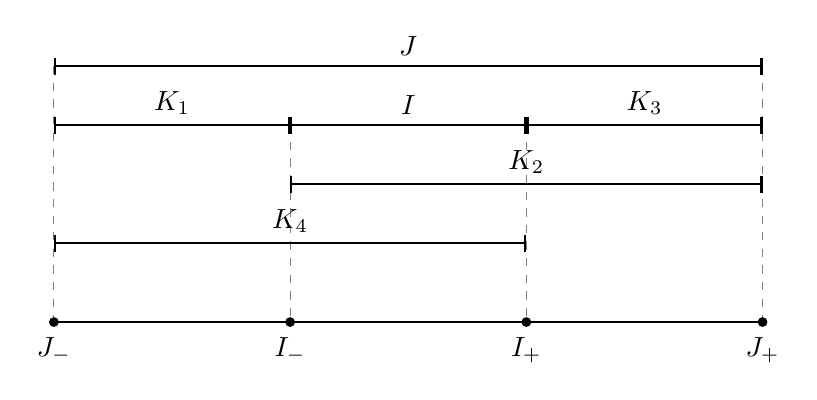
\begin{tikzpicture}
          \draw[dashed, color=gray, -] (0,0) -- (0, -3.25);
          \draw[dashed, color=gray, -] (3,-0.75) -- (3, -3.25);
          \draw[dashed, color=gray, -] (6,-0.75) -- (6, -3.25);
          \draw[dashed, color=gray, -] (9,0) -- (9, -3.25);

          \draw [thin,-] (0,-3.25) -- (9,-3.25);
          \node[circle,fill,inner sep=1.25pt,label=below:$\istart{J}$] (1) at (0,-3.25)  {};
          \node[circle,fill,inner sep=1.25pt,label=below:$\istart{I}$] (2) at (3,-3.25)  {};
          \node[circle,fill,inner sep=1.25pt,label=below:$\iend{I}$] (3) at (6,-3.25) {};
          \node[circle,fill,inner sep=1.25pt,label=below:$\iend{J}$] (3) at (9,-3.25) {};

          \draw[thick, |-|] (0,0) -- (9,0) node[above, midway] {$J$};
          \draw[thick, |-|] (3,-0.75) -- (6,-0.75) node[above, midway] {$I$};
          \draw[thick, |-|] (0,-0.75) -- (3,-0.75) node[above, midway] {$K_1$};
          \draw[thick, |-|] (6,-0.75) -- (9,-0.75) node[above, midway] {$K_3$};
          \draw[thick, |-|] (3,-1.5)  -- (9,-1.5) node[above, midway] {$K_2$};
          \draw[thick, |-|] (0,-2.25)  -- (6,-2.25) node[above, midway] {$K_4$};
        \end{tikzpicture}
      \end{center}
      This gives 4 intervals which all lie in the image of the unit
      \begin{align*}
        (\istart{J},\istart{I}) = \unit{A}(K_1) \qquad\qquad (\istart{J},\iend{I}) = \unit{A}(K_4) \\
        (\istart{I},\iend{J}) = \unit{A}(K_2)   \qquad\qquad (\iend{I},\iend{J}) = \unit{A}(K_3)
      \end{align*}
  \end{itemize}
  This is sufficient to see that $\unit{A}$ is surjective. After all fix some arbitrary interval
  \begin{equation*}
    ([(n,I)], [(m,J)]) \in \inter[\points[A]]
  \end{equation*}
  If $I = J$ then we must have
  \begin{equation*}
    ([(n,I)], [(m,J)]) = (\istart{I}, \iend{I}) = \unit{A}(I)
  \end{equation*}
  If $I \neq J$, then after possibly swapping $I,J$ we may assume $I \aiaarrow{<mosfd}$, which
  brings us to one of the cases handled above, where all intervals involing $\istart{I}, \iend{I},
  \istart{J}$ and $\iend{J}$ were in the image of the unit.
\end{proof}


\begin{cor}
  There exists an equivalence of categories between the full subcategory of strict linear orders $L$
  with $|L| \neq 1$ and the full subcategory of interval algebras satisfying $\allints$.
\end{cor}
\begin{proof}
  An adjunction can always be restricted to an equivalence of categories by considering the full
  subcategories where the unit and counit are isomorphisms.
\end{proof}

\newpage
\section{The Model Theory of Interval Algebras}
\label{sec:model_theory}

\subsection{The Fraïssé Class of Finite Interval Algebras}

We start by considering the class $\finaia$ of finite interval algebras. From our work in
\cref{ssub:homogeneous_structures_and_fraisse_classes}, we know that $\finaia$ satisfies the HP,
since $\taia$ is universal and relational. $\laia$ is also finite, so $\finaia$ must be EC.

To prove that $\finaia$ has the JEP and AP, notice that $\points$ must send finite interval algebras
to finite strict linear orders. In fact, given an interval algebra $A$, $|\points[A]| \leq 2|A|$
since $\points[A]$ is a quotient of $A + A$. Similarly, $\inter$ must also send finite strict linear
orders to finite interval algebras as given a strict linear order $L$,
$|\inter[L]| = \binom{|L|}{2}$. Using this fact, we will be able to reduce the proof of these
properties to the proof that $\finslo$ satisfies them.

\begin{prop}
  The class $\finaia$ has the joint embedding property.
\end{prop}
\begin{proof}
  Given two finite interval algebras $A$ and $B$, we use the JEP of strict
  linear orders to get the following diagram in $\slos$
  \[\begin{tikzcd}
    {\points[A]} \\
    && \Omega \\
    {\points[B]}
    \arrow["f", from=1-1, to=2-3]
    \arrow["g"', from=3-1, to=2-3]
  \end{tikzcd}\]
  Then, applying $\inter$ and using the adjunction unit $\eta$, we get
  % https://q.uiver.app/?q=WzAsNSxbMiwwLCJcXGludGVyW1xccG9pbnRzW0FdXSJdLFsyLDIsIlxcaW50ZXJbXFxwb2ludHNbQl1dIl0sWzQsMSwiXFxpbnRlcltcXE9tZWdhXSJdLFswLDAsIkEiXSxbMCwyLCJCIl0sWzAsMiwiXFxpbnRlcltmXSIsMCx7ImNvbG91ciI6WzAsNjAsNjBdfSxbMCw2MCw2MCwxXV0sWzEsMiwiXFxpbnRlcltnXSIsMix7ImNvbG91ciI6WzAsNjAsNjBdfSxbMCw2MCw2MCwxXV0sWzQsMSwiXFx1bml0e0J9IiwyXSxbMywwLCJcXHVuaXR7QX0iXV0=
  \[\begin{tikzcd}
    A && {\inter[\points[A]]} \\
    &&&& {\inter[\Omega]} \\
    B && {\inter[\points[B]]}
    \arrow["{\inter[f]}", color={rgb,255:red,214;green,92;blue,92}, from=1-3, to=2-5]
    \arrow["{\inter[g]}"', color={rgb,255:red,214;green,92;blue,92}, from=3-3, to=2-5]
    \arrow["{\unit{B}}"', from=3-1, to=3-3]
    \arrow["{\unit{A}}", from=1-1, to=1-3]
  \end{tikzcd}\]
  And the composites $\inter[f] \circ \unit{A}$ and $\inter[g] \circ \unit{B}$ along with
  the interval algebra $\Omega$ give us the joint embedding of $A$ and $B$.
\end{proof}

\begin{prop}
  The class $\finaia$ has the amalgamation property.
\end{prop}
\begin{proof}
  Suppose we have the following diagram in $\aias$
  % https://q.uiver.app/?q=WzAsNCxbMiwwLCJBIl0sWzIsMiwiQiJdLFswLDEsIkMiXSxbNCwxXSxbMiwwLCJmIl0sWzIsMSwiZyIsMl1d
  \[\begin{tikzcd}
    && A \\
    C &&&& {} \\
    && B
    \arrow["f", from=2-1, to=1-3]
    \arrow["g"', from=2-1, to=3-3]
  \end{tikzcd}\]
  Applying $\points$ takes us to $\slos$, at which point we can use the AP of strict linear
  orders to get the commuting square
  % https://q.uiver.app/?q=WzAsNCxbMiwwLCJcXHBvaW50c1tBXSJdLFsyLDIsIlxccG9pbnRzW0JdIl0sWzAsMSwiXFxwb2ludHNbQ10iXSxbNCwxLCJcXE9tZWdhIl0sWzIsMCwiXFxwb2ludHNbZl0iLDAseyJjb2xvdXIiOlswLDYwLDYwXX0sWzAsNjAsNjAsMV1dLFsyLDEsIlxccG9pbnRzW2ddIiwyLHsiY29sb3VyIjpbMCw2MCw2MF19LFswLDYwLDYwLDFdXSxbMCwzLCJmJyJdLFsxLDMsImcnIiwyXV0=
  \[\begin{tikzcd}
    && {\points[A]} \\
    {\points[C]} &&&& \Omega \\
    && {\points[B]}
    \arrow["{\points[f]}", color={rgb,255:red,214;green,92;blue,92}, from=2-1, to=1-3]
    \arrow["{\points[g]}"', color={rgb,255:red,214;green,92;blue,92}, from=2-1, to=3-3]
    \arrow["{f'}", from=1-3, to=2-5]
    \arrow["{g'}"', from=3-3, to=2-5]
  \end{tikzcd}\]
  Now going back to $\aias$ gives the commuting diagram
  % https://q.uiver.app/?q=WzAsOSxbNCwwLCJcXGludGVyW1xccG9pbnRzW0FdXSJdLFs0LDIsIlxcaW50ZXJbXFxwb2ludHNbQl1dIl0sWzIsMSwiXFxpbnRlcltcXHBvaW50c1tDXV0iXSxbNiwxLCJcXGludGVyW1xcT21lZ2FdIl0sWzAsMSwiQyJdLFswLDBdLFsxLDBdLFsyLDAsIkEiXSxbMiwyLCJCIl0sWzIsMCwiXFxpbnRlcltcXHBvaW50c1tmXV0iLDEseyJjb2xvdXIiOlswLDYwLDYwXX0sWzAsNjAsNjAsMV1dLFsyLDEsIlxcaW50ZXJbXFxwb2ludHNbZ11dIiwxLHsiY29sb3VyIjpbMCw2MCw2MF19LFswLDYwLDYwLDFdXSxbMCwzLCJcXGludGVyW2YnXSIsMCx7ImNvbG91ciI6WzAsNjAsNjBdfSxbMCw2MCw2MCwxXV0sWzEsMywiXFxpbnRlcltnJ10iLDIseyJjb2xvdXIiOlswLDYwLDYwXX0sWzAsNjAsNjAsMV1dLFs4LDEsIlxcdW5pdHtCfSIsMl0sWzcsMCwiXFx1bml0e0F9Il0sWzQsMiwiXFx1bml0e0N9IiwxXSxbNCw3LCJmIl0sWzQsOCwiZyIsMl1d
  \[\begin{tikzcd}
    {} & {} & A && {\inter[\points[A]]} \\
    C && {\inter[\points[C]]} &&&& {\inter[\Omega]} \\
    && B && {\inter[\points[B]]}
    \arrow["{\inter[\points[f]]}"{description}, color={rgb,255:red,214;green,92;blue,92}, from=2-3, to=1-5]
    \arrow["{\inter[\points[g]]}"{description}, color={rgb,255:red,214;green,92;blue,92}, from=2-3, to=3-5]
    \arrow["{\inter[f']}", color={rgb,255:red,214;green,92;blue,92}, from=1-5, to=2-7]
    \arrow["{\inter[g']}"', color={rgb,255:red,214;green,92;blue,92}, from=3-5, to=2-7]
    \arrow["{\unit{B}}"', from=3-3, to=3-5]
    \arrow["{\unit{A}}", from=1-3, to=1-5]
    \arrow["{\unit{C}}"{description}, from=2-1, to=2-3]
    \arrow["f", from=2-1, to=1-3]
    \arrow["g"', from=2-1, to=3-3]
  \end{tikzcd}\]
  For the AP of the finite interval algebras, we are only interested in the outer square. The
  necessary maps are then $\inter[f'] \circ \unit{A}$ and $\inter[g'] \circ \unit{B}$, both
  mapping into $\inter[\Omega]$.
\end{proof}

\begin{thm}
  The Fraïssé limit of $\finaia$ is $\inter[\Q]$
\end{thm}
\begin{proof}
  To show that the Fraïssé limit of the finite interval algebras is $\inter[\Q]$, it suffices to
  show that $\age(\inter[\Q]) = \finaia$ and that $\inter[\Q]$ is homogeneous.

  To see that $\age(\inter[\Q]) = \finaia$, prove that both sides include into the other.
  Suppose we have some finitely generated $\laia$-substructure $A \subset \inter[\Q]$. Since
  $\taia$ is universal, $A$ must also be an interval algebra. Furthermore, since $\laia$ is
  relational, $A$ must also be finite, so $A \in \finaia$. For the converse inclusion, consider
  some finite interval algebra $A$, it must embed into $\inter[\points[A]]$, which in turn
  embeds into $\inter[\Q]$ (since $\points[A]$ is finite, hence embeddable into $\Q$).
  Restricting these composition of these embeddings onto their image in $\inter[\Q]$ then gives
  the needed isomorphism.

  As for why $\inter[\Q]$ is homogeneous, fix two $\laia$-substructures $A,B \subseteq \inter[\Q]$,
  along with some $\laia$-isomorphism $f : A \to B$. In essence we have the following
  diagram of interval algebras, where $i$ and $j$ are the inclusions into $\inter[\Q]$:
  % https://q.uiver.app/?q=WzAsNCxbMCwyLCJBIl0sWzIsMiwiQiJdLFswLDAsIlxcaW50ZXJbXFxRXSJdLFsyLDAsIlxcaW50ZXJbXFxRXSJdLFswLDEsImYiXSxbMCwyLCJpIl0sWzEsMywiaiIsMl1d
  \[\begin{tikzcd}
    {\inter[\Q]} && {\inter[\Q]} \\
    \\
    A && B
    \arrow["f", from=3-1, to=3-3]
    \arrow["i", from=3-1, to=1-1]
    \arrow["j"', from=3-3, to=1-3]
  \end{tikzcd}\]
  Applying $\inter$ to move to linear orders, we can postcompose $\points[i]$ and $\points[j]$ with
  the counit at $\Q$ to realise $\points[A]$ and $\points[B]$ as $\lslo$-substructures of $\Q$.
  Now, $\points[f]$ is still an isomorphism as these are preserved by functors, and using the
  fact that $\Q$ is homogeneous, we can extend $\points[f]$ to an isomorphism $g$, giving the
  commuting diagram
  % https://q.uiver.app/?q=WzAsNyxbMCw0LCJcXHBvaW50c1tBXSJdLFsyLDQsIlxccG9pbnRzW0JdIl0sWzAsMiwiXFxwb2ludHNbXFxpbnRlcltcXFFdXSJdLFsyLDIsIlxccG9pbnRzW1xcaW50ZXJbXFxRXV0iXSxbMCwwLCJcXFEiXSxbMiwwLCJcXFEiXSxbMCwxXSxbMCwxLCJcXHBvaW50c1tmXSIsMCx7ImNvbG91ciI6WzAsNjAsNjBdfSxbMCw2MCw2MCwxXV0sWzAsMiwiXFxwb2ludHNbaV0iLDAseyJjb2xvdXIiOlswLDYwLDYwXX0sWzAsNjAsNjAsMV1dLFsyLDQsIlxcY291bml0e1xcUX0iXSxbMyw1LCJcXGNvdW5pdHtcXFF9IiwyXSxbMSwzLCJcXHBvaW50c1tqXSIsMix7ImNvbG91ciI6WzAsNjAsNjBdfSxbMCw2MCw2MCwxXV0sWzQsNSwiZyJdXQ==
  \[\begin{tikzcd}
    \Q && \Q \\
    {} \\
    {\points[\inter[\Q]]} && {\points[\inter[\Q]]} \\
    \\
    {\points[A]} && {\points[B]}
    \arrow["{\points[f]}", color={rgb,255:red,214;green,92;blue,92}, from=5-1, to=5-3]
    \arrow["{\points[i]}", color={rgb,255:red,214;green,92;blue,92}, from=5-1, to=3-1]
    \arrow["{\counit{\Q}}", from=3-1, to=1-1]
    \arrow["{\counit{\Q}}"', from=3-3, to=1-3]
    \arrow["{\points[j]}"', color={rgb,255:red,214;green,92;blue,92}, from=5-3, to=3-3]
    \arrow["g", from=1-1, to=1-3]
  \end{tikzcd}\]
  Finally, we apply $\inter$ to bring us back to interval algebras, where we have the following
  diagram:
  % If modifying diagram, don't forget to add [scale cd=0.91]
  % https://q.uiver.app/?q=WzAsMTIsWzIsNCwiXFxpbnRlcltcXHBvaW50c1tBXV0iXSxbNCw0LCJcXGludGVyW1xccG9pbnRzW0JdXSJdLFsyLDIsIlxcaW50ZXJbXFxwb2ludHNbXFxpbnRlcltcXFFdXV0iXSxbNCwyLCJcXGludGVyW1xccG9pbnRzW1xcaW50ZXJbXFxRXV1dIl0sWzIsMCwiXFxpbnRlcltcXFFdIl0sWzQsMCwiXFxpbnRlcltcXFFdIl0sWzQsNiwiQiJdLFsyLDYsIkEiXSxbNiwyLCJcXGludGVyW1xcUV0iXSxbMCwyLCJcXGludGVyW1xcUV0iXSxbMCw0LCJBIl0sWzYsNCwiQiJdLFswLDEsIlxcaW50ZXJbXFxwb2ludHNbZl1dIiwwLHsiY29sb3VyIjpbMCw2MCw2MF19LFswLDYwLDYwLDFdXSxbMSwzLCJcXGludGVyW1xccG9pbnRzW2ldXSIsMCx7ImNvbG91ciI6WzAsNjAsNjBdfSxbMCw2MCw2MCwxXV0sWzAsMiwiXFxpbnRlcltcXHBvaW50c1tpXV0iLDIseyJjb2xvdXIiOlswLDYwLDYwXX0sWzAsNjAsNjAsMV1dLFsyLDQsIlxcaW50ZXJbXFxjb3VuaXR7XFxRfV0iLDIseyJjb2xvdXIiOlswLDYwLDYwXX0sWzAsNjAsNjAsMV1dLFszLDUsIlxcaW50ZXJbXFxjb3VuaXR7XFxRfV0iLDAseyJjb2xvdXIiOlswLDYwLDYwXX0sWzAsNjAsNjAsMV1dLFs0LDUsIlxcaW50ZXJbZ10iLDAseyJjb2xvdXIiOlswLDYwLDYwXX0sWzAsNjAsNjAsMV1dLFs3LDAsIlxcdW5pdHtBfSIsMl0sWzYsMSwiXFx1bml0e0J9Il0sWzgsMywiXFx1bml0e1xcaW50ZXJbXFxRXX0iXSxbOSwyLCJcXHVuaXR7XFxpbnRlcltcXFFdfSIsMl0sWzgsNSwiXFxpZHtcXGludGVyW1xcUV19IiwyLHsiY3VydmUiOjN9XSxbOSw0LCJcXGlke1xcaW50ZXJbXFxRXX0iLDAseyJjdXJ2ZSI6LTN9XSxbNyw2LCJmIiwyXSxbMTAsOSwiaSJdLFsxMCwwLCJcXHVuaXR7QX0iLDJdLFs3LDEwLCJcXGlke0F9IiwwLHsiY3VydmUiOi0zfV0sWzExLDgsImoiLDJdLFsxMSwxLCJcXHVuaXR7Qn0iXSxbNiwxMSwiXFxpZHtCfSIsMix7ImN1cnZlIjozfV1d
  \[\begin{tikzcd}[scale cd=0.91]
    && {\inter[\Q]} && {\inter[\Q]} \\
    \\
    {\inter[\Q]} && {\inter[\points[\inter[\Q]]]} && {\inter[\points[\inter[\Q]]]} && {\inter[\Q]} \\
    \\
    A && {\inter[\points[A]]} && {\inter[\points[B]]} && B \\
    \\
    && A && B
    \arrow["{\inter[\points[f]]}", color={rgb,255:red,214;green,92;blue,92}, from=5-3, to=5-5]
    \arrow["{\inter[\points[i]]}", color={rgb,255:red,214;green,92;blue,92}, from=5-5, to=3-5]
    \arrow["{\inter[\points[i]]}"', color={rgb,255:red,214;green,92;blue,92}, from=5-3, to=3-3]
    \arrow["{\inter[\counit{\Q}]}"', color={rgb,255:red,214;green,92;blue,92}, from=3-3, to=1-3]
    \arrow["{\inter[\counit{\Q}]}", color={rgb,255:red,214;green,92;blue,92}, from=3-5, to=1-5]
    \arrow["{\inter[g]}", color={rgb,255:red,214;green,92;blue,92}, from=1-3, to=1-5]
    \arrow["{\unit{A}}"', from=7-3, to=5-3]
    \arrow["{\unit{B}}", from=7-5, to=5-5]
    \arrow["{\unit{\inter[\Q]}}", from=3-7, to=3-5]
    \arrow["{\unit{\inter[\Q]}}"', from=3-1, to=3-3]
    \arrow["{\id{\inter[\Q]}}"', curve={height=18pt}, from=3-7, to=1-5]
    \arrow["{\id{\inter[\Q]}}", curve={height=-18pt}, from=3-1, to=1-3]
    \arrow["f"', from=7-3, to=7-5]
    \arrow["i", from=5-1, to=3-1]
    \arrow["{\unit{A}}"', from=5-1, to=5-3]
    \arrow["{\id{A}}", curve={height=-18pt}, from=7-3, to=5-1]
    \arrow["j"', from=5-7, to=3-7]
    \arrow["{\unit{B}}", from=5-7, to=5-5]
    \arrow["{\id{B}}"', curve={height=18pt}, from=7-5, to=5-7]
  \end{tikzcd}\]
  Although not obvious at first, the above diagram commutes, to check this we look at all the
  "irreducible components" individually:
  \begin{itemize}
    \item The middle rectangle in red commutes since it already commuted for linear orders.
    \item The top triangles commute by triangle identities of our adjunction.
    \item The squares to the left, right and bottom of the red rectangle commute by naturality
      of the unit.
    \item The bottom triangles commute due to the use of the identity.
  \end{itemize}
  Chasing around the outside of the diagram, we see that
  \begin{equation*}
    \inter[g] \circ \id{\inter[\Q]} \circ i \circ \id{A} =
      \id{\inter[\Q]} \circ j \circ \id{B} \circ f
  \end{equation*}
  Simplifying by removing identities shows that $\inter[g] \circ i = j \circ f$. Now, since $g$
  was an isomorphism, so is $\inter[g]$, so we have successfully extended $f$ to an
  automorphism of $\inter[\Q]$.
\end{proof}

\subsection{Stable and NIP Interval Agebras}

The question of stability for interval algebras is answered similarly to linear orders, as only the
finite interval algebras are stable.

\begin{thm}
  An interval algebra $A$ is stable if and only if it is finite.
\end{thm}
\begin{proof}
  Suppose that $A$ is an interval algebra and consider the formula
  \begin{equation*}
    \lexord(I, J) = (I \before J) \lor (I \meets J) \lor (I \overlaps J) \lor (I \starts J)
                                  \lor (I \finishedby J) \lor (I \contains J)
  \end{equation*}
  The above formula takes the elements of $A$ and lexicographically orders them, by first comparing
  the start times of each interval, and then the end times if the start times coincide. As a
  result, the formula $\lexord$ gives the structure of a strict linear order to the elements
  of $A$:
  \begin{itemize}
    \item \textbf{irreflexivity}: Fix some interval $I \in A$, then $I = I$. Since the relational
      symbols of interval algebras along with equality are all mutually exclusive,
      neither $I \aiaarrow{i} I$ nor $I \raiaarrow{i} I$ can hold for any $i \in \aiaindex$. This
      means $A \models \lnot \lexord(I, I)$ so $\lexord$ is irreflexive.
    \item \textbf{transitivity}: Fix three intervals $I,J,K \in A$ and suppose that
      $A \models \lexord(I,J)$ and $A \models \lexord(J,K)$. Since $\lexord$ consists of the disjunction of 6
      relational symbols, there are 36 cases which would lead to this situation. Considering each of
      these cases individually and looking up our transitivity axioms for interval algebras, we can
      find all possible relations between $I$ and $K$, which is detailed in \cref{tab:lexord_trans}.
      In all of these cases, we must still have $A \models \lexord(I,K)$, so
      $\lexord$ is transitive.
    \item \textbf{trichotomy}: Fix two intervals $I, J \in A$. First notice that
      $A \models \lexord(J,I)$ if and only if we have
      \begin{equation*}
        A \models (I \after J) \lor (I \metby J) \lor (I \overlappedby J) \lor (I \startedby J)
                      \lor (I \finishes J) \lor (I \contained J)
      \end{equation*}
      which is the same as taking the dual of all the relation symbols in $\lexord(I,J)$.
      Hence $A \models \lexord(I,J) \lor (I = J) \lor \lexord(J,I)$ is equivalent to saying that
      the interval algebra relations are exhaustive, which is one of our axioms. Hence the strict
      ordering given by $\lexord$ is linear.
  \end{itemize}

  \transreltable{lexord_trans}{Cases for transitivy of $\lexord$.}{
    \llrow & \slrow \\
    \lmrow & \smrow \\
    \lorow & \sorow \\
    \lsrow & \ssrow \\
    \lFrow & \sFrow \\
    \lDrow & \sDrow \\
    \hline
    \mlrow & \Flrow \\
    \mmrow & \Fmrow \\
    \morow & \Forow \\
    \msrow & \Fsrow \\
    \mFrow & \FFrow \\
    \mDrow & \FDrow \\
    \hline
    \olrow & \Dlrow \\
    \omrow & \Dmrow \\
    \oorow & \Dorow \\
    \osrow & \Dsrow \\
    \oFrow & \DFrow \\
    \oDrow & \DDrow \\
  }

  Now for any finite interval algebra $A$, all strict linear orders interpretable in $A$ will be
  bounded in size by $|A|^k$ for some $k \in \N$. In particular, all such linear orders must be
  finite, so $A$ is stable.

  For the converse, suppose $A$ is stable. Using $\lexord$ we can linearly order all the elements
  of $A$, but as $A$ is stable this linear order must be finite, hence $A$ must be finite.
\end{proof}

Restricting our attention to interval algebras with all possible intervals, the question of which
interval algebras are NIP has an answer similar to the linear order case.

\begin{thm}
  For any linear order $L$, the interval algebra $\inter[L]$ is NIP.
\end{thm}
\begin{proof}
  Suppose that $\inter[L]$ has the IP, so there is some formula $\phi(x;y)$ which has the IP. Let
  the IP of $\phi(x;y)$ be realised by the model $A \models \fulltheory(\inter[L])$ and sequences
  $(a_i)_{i < \omega}$ and $(b_I)_{I \subseteq \omega}$. Since finite interval algebras are stable
  and hence NIP, we may assume that $L$ is infinite, so
  the counit $\counit{L}$ is an isomorphism. By the triangle laws of our adjunction we know that
  \begin{equation*}
    \inter[\counit{L}] \circ \unit{\inter[L]} = \id{\inter[L]}
  \end{equation*}
  As $\counit{L}$ is an isomorphism, $\inter[\counit{L}]$ must also be an isomorphism, so
  $\unit{\inter[L]}$ too is an isomorphism. In particular, this implies that
  $\inter[L] \models \allints$. As a result, $A \models \allints$ too and $A \cong \inter[L']$ for
  some strict linear order $L'$. Recall that $\inter[L']$ is interpretable in $L'$, hence we can
  translate the formula $\phi(x;y)$ to some formula $\phi'(x;y)$ in the language of strict linear
  orders. In addition, we can also translate the sequences of tuples $(a_i)_{i < \omega}$ and
  $(b_I)_{I \subseteq \omega}$ to sequences of tuples in $L'$. This means that the formula
  $\phi'(x;y)$ has the IP, making the linear order $L'$ also have the IP. This is a contradiction as
  all linear orders have the NIP, so $\inter[L]$ must also have the NIP.
\end{proof}

However, as we saw before with the exponential fields case, by modifying models even slightly we can
add enough expressive power to get the IP. Likewise, by starting with an interval algebra with the
NIP, we can remove enough intervals to allow for the IP.

\begin{exmp}
  Let $L = \R \sqcup \N$ be the linear order given by putting all the elements of $\R$ before $\N$.
  By picking out the right substructure $A \subseteq \inter[L]$ we should get an interval algebra
  with the IP.

  First fix some bijection $f : \PS(\N) \overset{\sim}{\longrightarrow} \R$ and then let $A$ be the
  substructure of $\inter[L]$ given by
  \begin{align*}
    A = & \left\{ (x,y) \ \big|\ x,y \in \R \text{ such that } x < y \right\} \\
        & \qquad \cup \left\{ (f(I),i) \ \big|\ I \subseteq \N, i \in I \right\} \\
        & \qquad \cup \left\{ (x,y)\ \big|\ x,y \in \N \text{ such that } x < y \right\}
  \end{align*}
  In particular, the only intervals $(x,a) \in A$ with $x \in \R$ and $a \in \N$ come from the
  set comprehension $\left\{ (f(I),i) \ \big|\ I \subseteq \N, i \in I \right\}$. Using
  $I_{S}$ to denote the interval $(f(S)-1,f(S)$ and $J_n$ to denote $(n,n+1)$, we would end
  up with something like
  \begin{center}
    \begin{tikzpicture}
      \path (-1,0) -- node[auto=false]{$\ldots$} (0,0);
      \draw [thin,-] (0,0) to node[above] {$\R$} (4,0);
      \path (4,0) -- node[auto=false]{$\ldots$} (5,0);
      \draw [thin,-] (6,0) to node[above] {$\N$} (11,0);
      \path (11,0) -- node[auto=false]{$\ldots$} (12,0);

      \draw[thin,|-|] (2.75,-1) to node[above] {$I_{\{0\}}$} (3.75,-1);
      \draw[thin,|-|] (3.75,-1) to node[above] {} (6,-1);
      \draw[thin,|-|] (6,-1) to node[above] {$J_0$} (7,-1);

      \draw[thin,|-|] (0.5,-1.75) to node[above] {$I_{\{1,2\}}$} (1.5,-1.75);
      \draw[thin,|-|] (1.5,-1.75) to node[above] {} (7,-1.75);
      \draw[thin,|-|] (7,-1.75) to node[above] {$J_1$} (8,-1.75);
      \draw[thin,|-|] (1.5,-2.5) to node[above] {} (8,-2.5);
      \draw[thin,|-|] (8,-2.5) to node[above] {$J_2$} (9,-2.5);
    \end{tikzpicture}
  \end{center}

  Now the formula
  \begin{equation*}
    \phi(I;J) = \exists K,\; (J \meets K) \land (K \meets I)
  \end{equation*}
  has the IP and this is realised in $A$ by the sequences $(a_i)_{i \in \N}$ and
  $(b_I)_{I \subseteq \N}$ defined by
  \begin{equation*}
    a_i = (i, i+1) \qquad\qquad b_I = (f(I) - 1, f(I))
  \end{equation*}
  Since for any $i \in \N$ and $I \subseteq \N$, $A \models \phi(a_i, b_I)$ if and only if there
  exists some interval $(x,y) \in A$ with $x,y \in L$ such that
  \begin{equation*}
    (f(I) - 1, f(I)) \meets (x,y) \land (x,y) \meets (i, i + 1)
  \end{equation*}
  This can only happen if $x = f(I)$ and $y = i$, so we would require
  \begin{equation*}
    (f(I), i) \in \left\{ (f(I),i) \ \big|\ I \subseteq \N, i \in I \right\}
  \end{equation*}
  which happens if and only if $i \in I$ as needed.
\end{exmp}


\newpage
\section{Evaluation}

At the start of this project we had one overarching objective, that was to come up with some axioms
for the theory of interval algebras and study their model theoretic consequences.
As such the main topic of concern for our evaluation will be deciding how appropriate our
axiomatisation was.

Firstly, we should consider the models allowed by our axiomatisation. We saw that the models of
$\taia$ coincide with the class of substructures of the interval algebras $\inter[L]$.
These are exactly the type of models that underlie the work in \cite{allen83}, on this front
we should be very happy with our axiomatisation. In addition, we also saw that
$\taia \cup \{\allints\}$ axiomatised the class of models of the form $\inter[L]$, letting us
distinguish an important class of models through a single sentence.

In addition, $\taia$ is also finite, meaning there is very little ambiguity when checking
whether a structure is a model or not. On the other hand, despite being finite, there are quite
a lot of axioms in $\taia$ due to its many relations. This means proving things about
interval algebras can be quite labourious, with a lot of quite distinct cases to check. If we could
find some symmetry in the transitivity relations this would help a lot, but there does not seem
to be anything too tangible to simplify reasoning.

Finally, with our given axioms, we managed to prove all of the results we were originally
interested at the start of this project, so our axiomatisation was definitely something we could
work with.

\newpage
\section{Conclusion}
\label{sec:conclusion}

We started this report by establishing a list of axioms for the theory of interval algebras, which
we showed to be satisfiable, containing at least the main class of models we expected. Then,
through further study of the interval construction, we saw it to be a right adjoint. The unit of
this adjunction then meant that every model was a substructure of the intervals over an appropriate
linear order, cementing the relevancy of our axiomatisation.

In attempting to characterise the interval algebras for which the unit was an isomorphism, we found
a formula $\allints$ axiomatising the interval algebras of the form $\inter[L]$. Since the interval
algebra $\inter[L]$ can always be interpretable in $L$, this meant that $\inter[L]$ always has the
NIP.

This is where our work finishes, but there are some possibilities for future work.

First, suppose that we removed the $I \before J$ conjunct from $\allints$ to get
\begin{align*}
  \mostints = & \left(\forall I,\; \forall J,\;
        (I \meets J)     \rightarrow \exists K,\; (I \startedby K)  \land (K \finishes J) \right)\\
    & \land \left(\forall I,\; \forall J,\;
        (I \overlaps J)  \rightarrow \exists K,\; (I \finishedby K) \land (K \starts J)   \right)\\
    & \land \left(\forall I,\; \forall J,\;
        (I \starts J)    \rightarrow \exists K,\; (I \meets K)      \land (K \finishes J) \right)\\
    & \land \left(\forall I,\; \forall J,\;
        (I \finishes J)  \rightarrow \exists K,\; (I \metby K)      \land (K \starts J)   \right)\\
    & \land \left(\forall I,\; \forall J,\;
        (I \contained J) \rightarrow \exists K,\; (I \metby K)      \land (K \starts J)   \right)
\end{align*}
Then it would be interesting to see the type of interval algebras satisfying $\mostints$. We expect
such an interval algebra $A$ to look like a gluing of $\{ \inter[L_i] \}_{i \in I}$ where the
indexing set $I$ is linearly ordered. If this were true, then letting $L$ be the linear order
cosntructed by gluing $\{L_i\}_{i \in I}$, we would expect $A$ to be interpretable in the linear
order $L$ plus some colouring predicates. Since a linear order always has the NIP, regardless of the
number of colouring predicates, this would extend our result about NIP interval algebras.

Another question possibly worth considering further comes from our work done with the interval
construction, which we saw to be a right adjoint functor. From category theory we know that
right adjoints preserve limits, and dually that left adjoints preserve colimits. Work by
Caramello \cite{caramello08} shows how to realise the Fraïssé limit of a Fraïssé class as a
colimit in the language of category theory. So here we have a functor, $\inter$, preserving quite
a complicated colimit. This could hint at a couple of options: it might be the case that $\inter$ is
also a left adjoint functor, although if this is the case it would have to be some new functor
distinct from $\points$. Alternatively, there could be something specific about Fraïssé limits
which meant they should be preserved by right adjoints. In either case, it would be interesting to
see what develops.

\newpage
\bibliographystyle{unsrtnat}
\bibliography{refs}

\end{document}
